\chapter{Optimization Results}
\label{sec:optimization_results}
This chapter focuses on showing and analyzing the most interesting MAV designs
produced by the optimization tool. A short digression on platonic solid is first
needed in order to properly analyze the results. The optimal designs with an even number
of propellers are then described. Afterwards, the designs with an odd number of
propellers are shown. A comparison of the different optimal drone design is then
proposed. Finally, a few results of optimizations performed with the number of
propeller as an argument are presented.

\section{Platonic Solids}
\label{sec:platonic_solids}
Platonic solids are five regular and convex polyhedrons named after the
ancient Greek philosopher Plato to honor his memory \citep{noauthor_platonic_2018}.
The five platonic solids are:
{\small\begin{itemize}
\item The tetrahedron composed of four faces and four vertices (see \Cref{fig:tetrahedron}).
\item The octahedron composed of eight faces and six vertices (see \Cref{fig:octahedron}).
\item The cube composed of six faces and eight vertices (see \Cref{fig:cube}).
\item The icosahedron composed of twenty faces and twelve vertices.
\item The dodecahedron composed of twelve faces and twenty vertices.
\end{itemize}}
There is a angle that can be found at least in the
first three platonic solids. This angle is found between the horizontal plane and
the vertices of the polyhedron (see \Cref{fig:platonic_solid}). This angle find itself
in some of the obtained results. So in order to ensure simplicity,
in the rest of this work this angle will be referred to as the platonic solids angle
($\beta_{PS}$).

\begin{figure}[!h]
  \begin{subfigure}[b]{0.22\textwidth}
    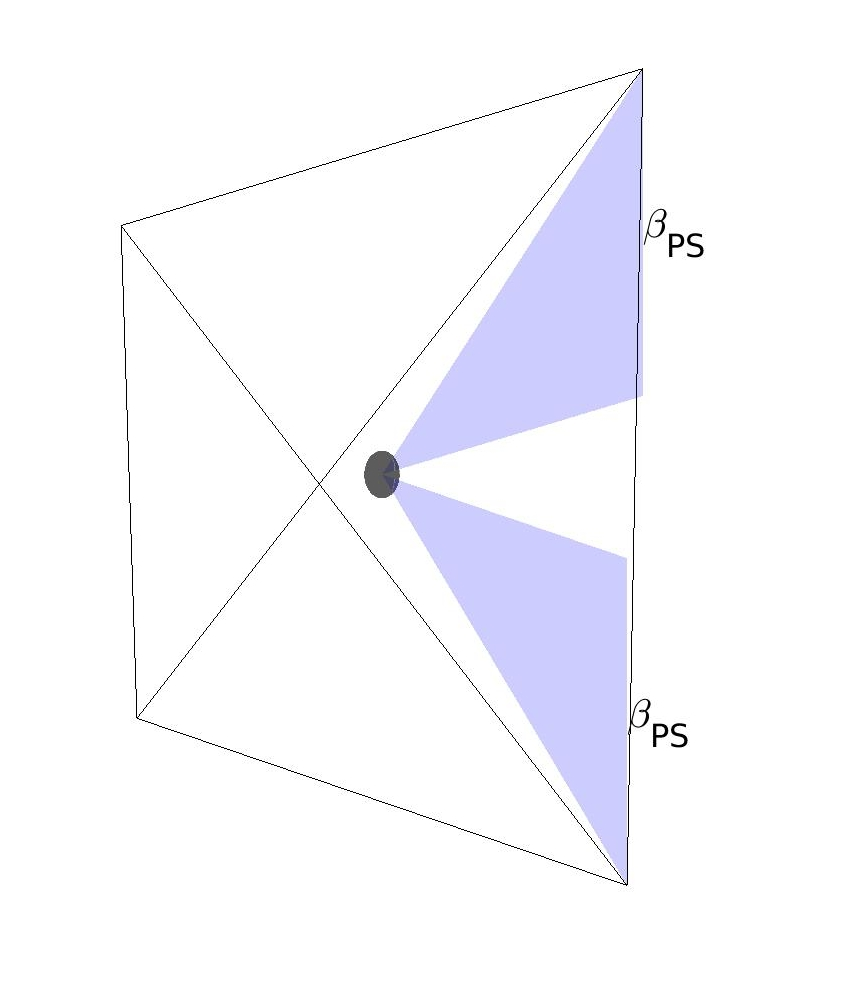
\includegraphics[width=\linewidth]{images/tetrahedron.jpg}
    \caption{Tetrahedron.} \label{fig:tetrahedron}
  \end{subfigure}
  \hspace*{\fill} % separation between the subfigures
  \begin{subfigure}[b]{0.27\textwidth}
    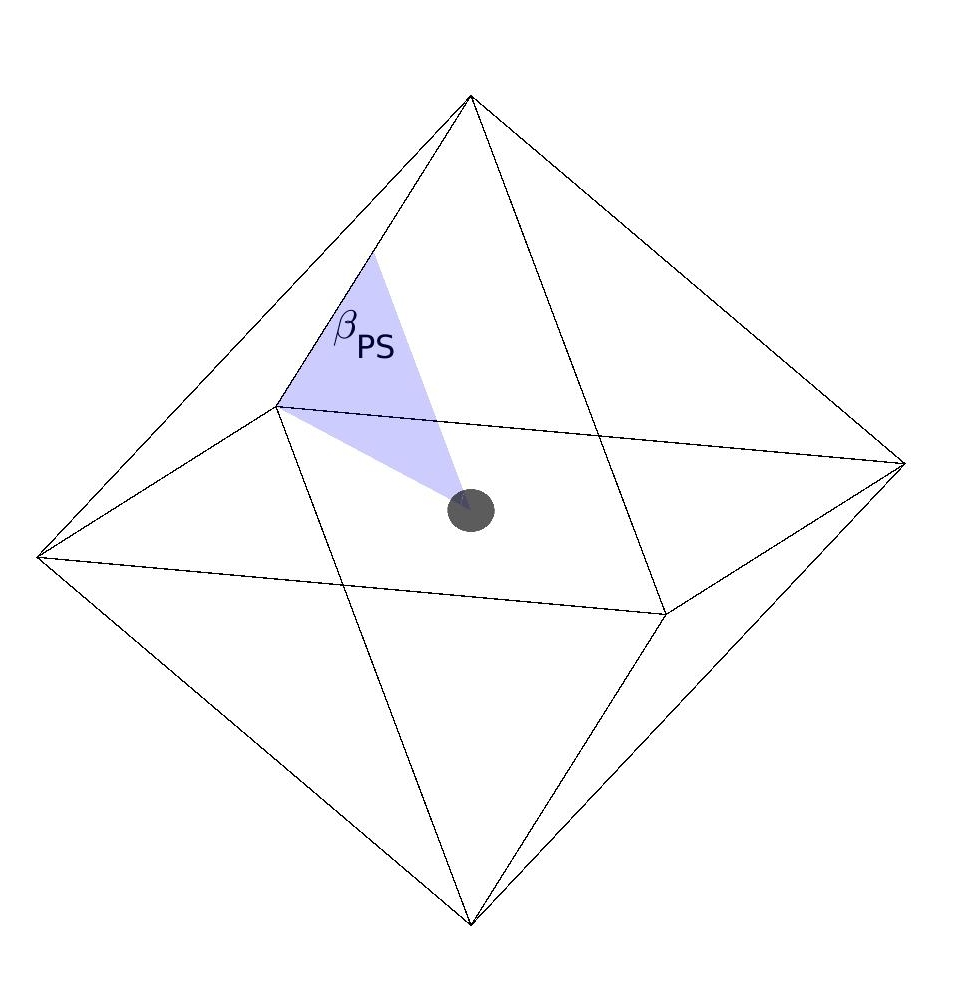
\includegraphics[width=\linewidth]{images/octahedron.jpg}
    \caption{Octahedron.} \label{fig:octahedron}
  \end{subfigure}
  \hspace*{\fill} % separation between the subfigures
  \begin{subfigure}[b]{0.26\textwidth}
    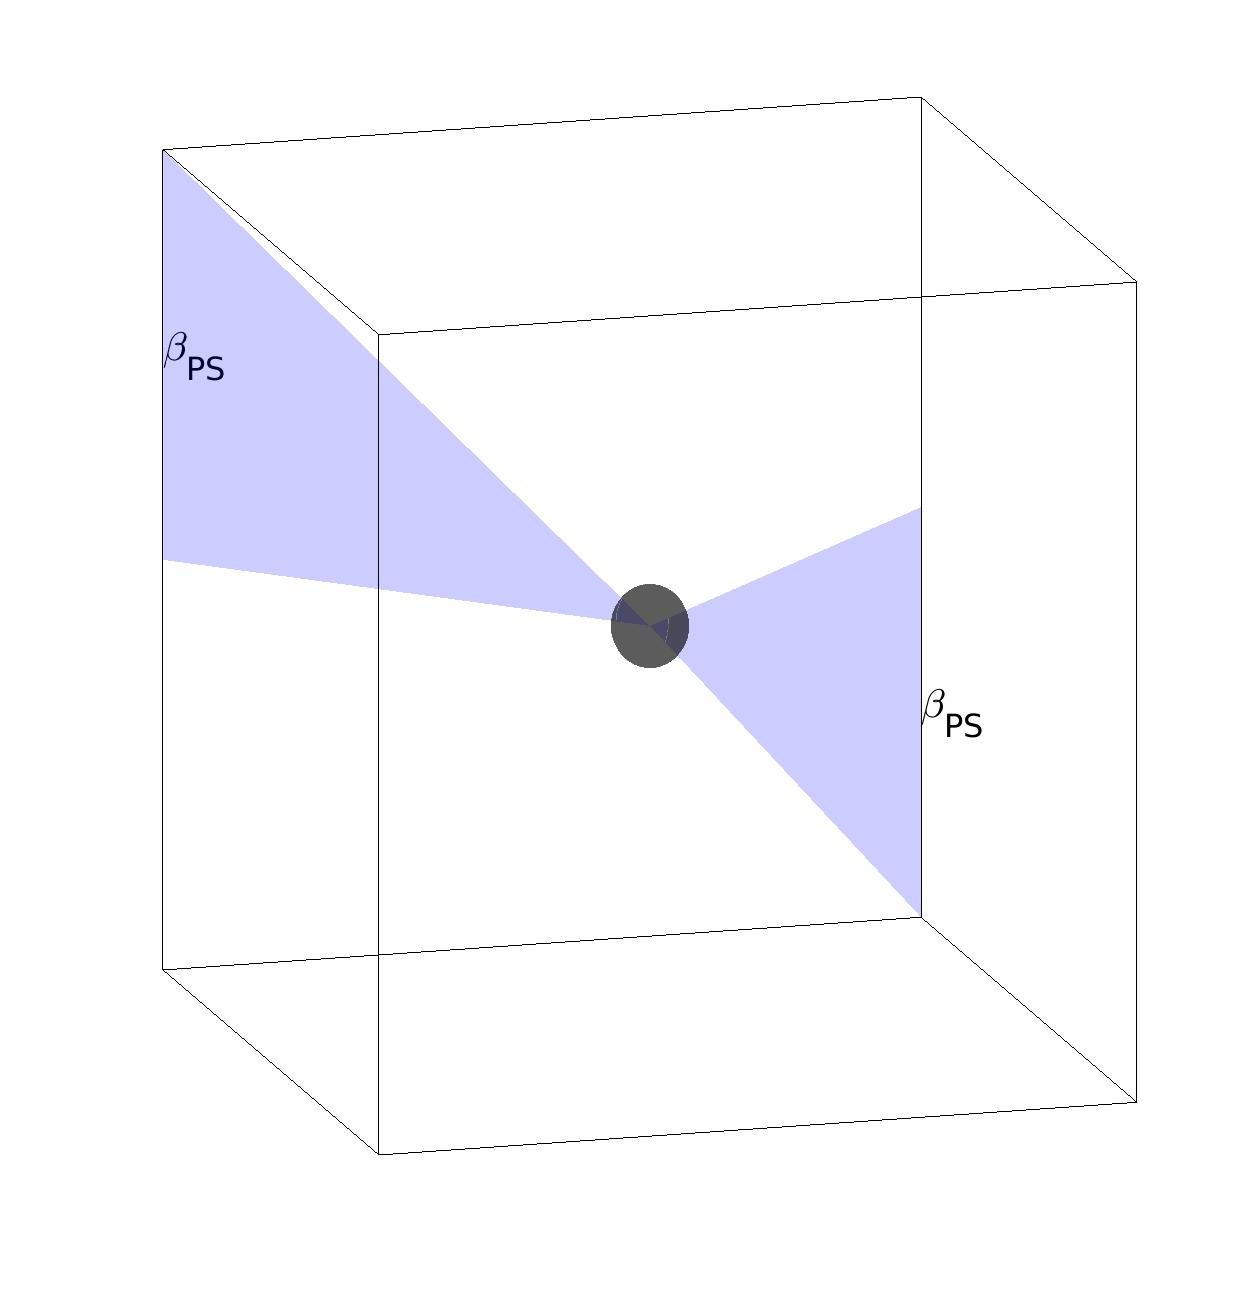
\includegraphics[width=\linewidth]{images/cube.jpg}
    \caption{Cube.} \label{fig:cube}
  \end{subfigure}
  \caption{The first three platonic solids $\big(\cos(\beta_{PS}) = \sqrt{\frac{2}{3}}
  \rightarrow \beta_{PS} \simeq 35.26^{\circ}\big)\, .$}
  \label{fig:platonic_solid}
\end{figure}

\section{Even Designs}
\label{sec:even_designs}
\subsection{Quad-copter}
\label{sec:quad_copter}
The first MAV morphology presented is obtained when optimizing to find
$\beta_{arm}$ and $\theta_{arm}$, with as fixed design parameters $n\ =\ 4$
and $L\ =\ 0.5\ [m]$ and as an initial solution $\beta_{arm,0} \ =\ [0^{\circ},
\  0^{\circ},\  0^{\circ},\ 0^{\circ}]$ and $\theta_{arm,0}\ =\
[0^{\circ},\  0^{\circ},\  0^{\circ},\  0^{\circ}]$. As a cost function for the
optimization problem, the cost function that maximizes the minimal attainable
force and the minimal attainable torque that the MAV can produce in any direction
and that minimizes the inertia of the drone is used. The result is depicted in
\Cref{fig:Quadcopter_1} and has the following features:
{\footnotesize\begin{itemize}
  \item $n\ =\ 4$
  \item $\beta_{arm}\ =\ [-32.42^{\circ},\  -35.49^{\circ},\  -35.44^{\circ},\  -35.49^{\circ}]$
  \item $\theta_{arm}\ =\ [-0.99^{\circ},\  -1.88^{\circ},\  -2.26^{\circ},\  -2.94^{\circ}]$
  \item $L\ =\ 0.5\ [m]$
\end{itemize}}
It is noticeable that the $\theta_{arm}$ tend towards zero and that the $\beta_{arm}$
tend towards the platonic solid angle $\beta_{PS}$. However, the design has not totally
converged. This is due to the fact that the optimization tool has, as mentioned in
\Cref{sec:limitations}, found a local minimum before reaching the global one,
which seems to be when the drone has the arms equally distributed in the horizontal
plane ($\theta_{arm}$ = 0) and forming the platonic solid angle with the same horizontal
plane ($\beta_{arm}\ =\ \beta_{PS}$). So as to verify this, the second
design is obtained when performing the same optimization as before with a slight
change, which consists in choosing as initial solution $\beta_{arm,0} \ =\
[35.26^{\circ},\  -35.26^{\circ},\  35.26^{\circ},\  -35.26^{\circ}]$. The result is
depicted in \Cref{fig:Quadcopter_1} and has the following features:
{\footnotesize\begin{itemize}
  \item $n\ =\ 4$
  \item $\beta_{arm}\ =\ [35.26^{\circ},\  -35.26^{\circ},\  35.26^{\circ},\  -35.26^{\circ}]$
  \item $\theta_{arm}\ =\ [0^{\circ},\  0^{\circ},\  0^{\circ},\  0^{\circ}]$
  \item $L\ =\ 0.5\ [m]$
\end{itemize}}
After optimization the second design is the same as the initial solution. This means
that the initially chosen design is optimal and it is very likely a global optimum
as when starting the optimization from different initial solution it converges to it.
It is interesting to note that the four propellers of the second design form the four
vertices of a tetrahedron (see \Cref{fig:Quadcopter_2_tetra}).
\begin{figure}[!h]
  \resizebox{\textwidth}{!}{\begin{subfigure}[b]{0.45\textwidth}
    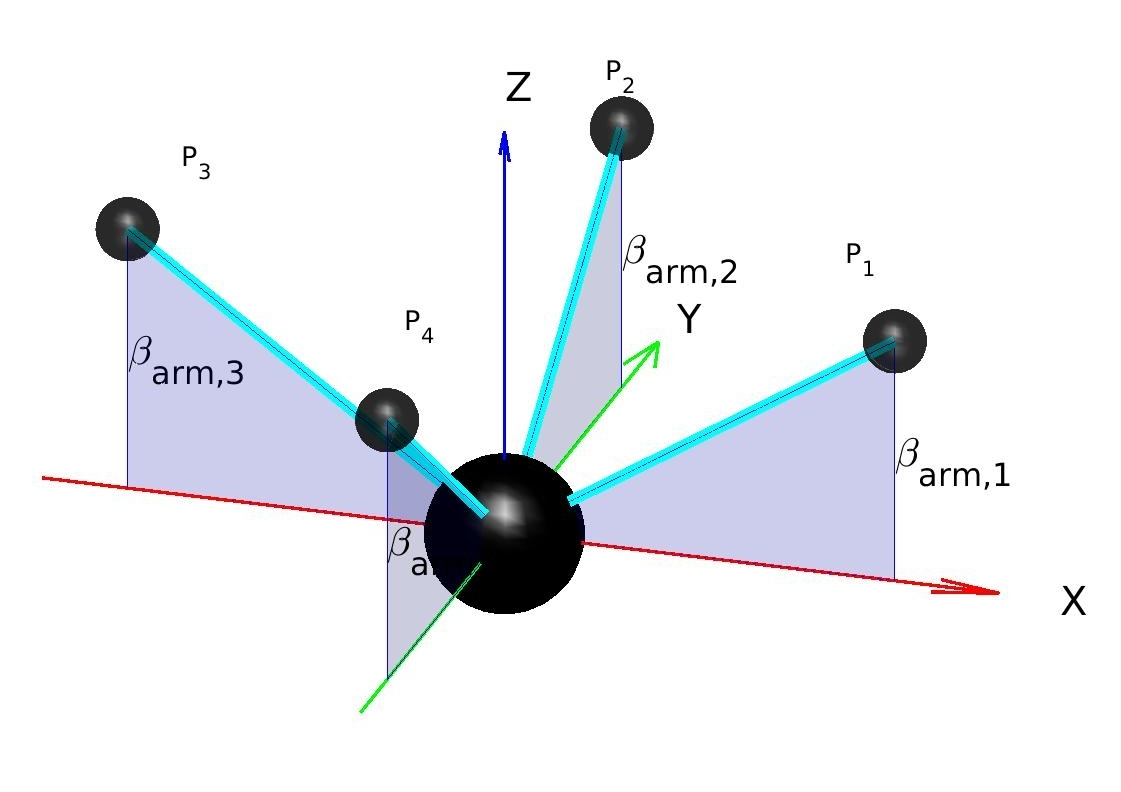
\includegraphics[width=\linewidth]{images/Quadcopter2.jpg}
    \caption{Design 1.} \label{fig:Quadcopter_1}
  \end{subfigure}
\hspace*{\fill} % separation between the subfigures
\begin{subfigure}[b]{0.4\textwidth}
    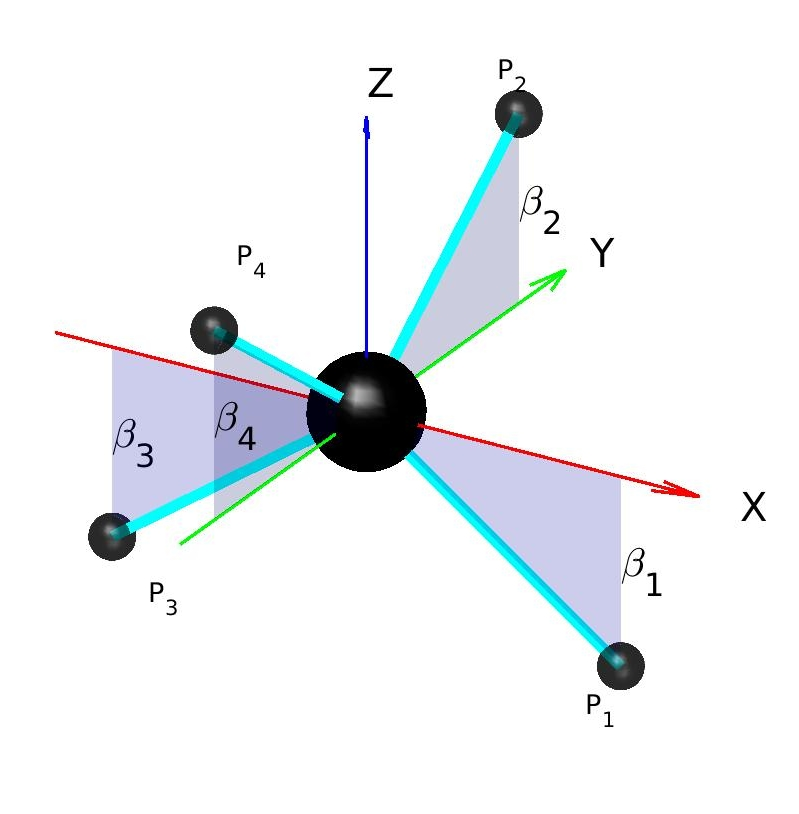
\includegraphics[width=\linewidth]{images/Quadcopter.jpg}
    \caption{Design 2.} \label{fig:Quadcopter_2}
  \end{subfigure}
  \hspace*{\fill} % separation between the subfigures
  \begin{subfigure}[b]{0.35\textwidth}
    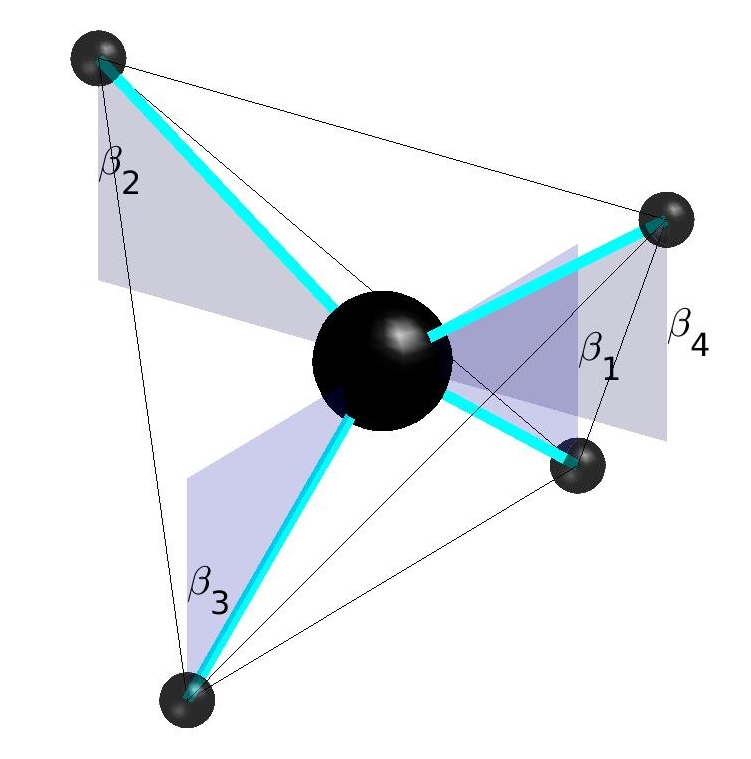
\includegraphics[width=\linewidth]{images/Quad_tetrahedron.jpg}
    \caption{Design 2 in a tetrahedron.} \label{fig:Quadcopter_2_tetra}
  \end{subfigure}}
  \caption{Schematic of the optimal designs obtained for the Quad-copter.}
  \label{fig:Quadcopter_result}
\end{figure}
It is important to understand that for the tool, the designs with all the arms
on the same side (as design 1), or the designs with distributed arms (as design 2),
are equivalent. Even with slightly different arm angles’ magnitudes
between the two designs, when comparing \Cref{fig:Quadcopter1_spaces}with
\Cref{fig:Quadcopter2_spaces} and when comparing the different metrics
in \Cref{tab:tab_Quad_compare_force}, \Cref{tab:tab_Quad_compare_torque} and
\Cref{tab:tab_Quad_compare_hover}, one can easily see that the two designs
propose similar abilities. The main difference is the location of their center of mass
that the tool does not consider. For instance, second design’s CoM coincide with
the body origin. Which renders the drone more balanced and thus more controllable.

\begin{figure}[!h]
  \resizebox{\textwidth}{!}{\begin{subfigure}[b]{0.55\textwidth}
    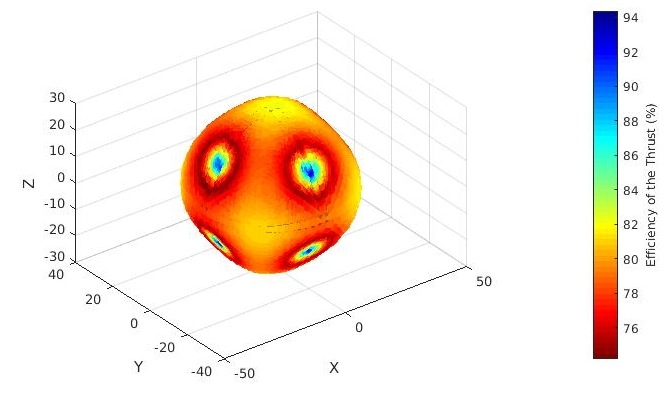
\includegraphics[width=\linewidth]{images/Quad_design_2_fspace.jpg}
    \caption{Attainable force space.} \label{fig:deisgn1_fspace}
  \end{subfigure}
  \hspace*{\fill} % separation between the subfigures
  \begin{subfigure}[b]{0.51\textwidth}
    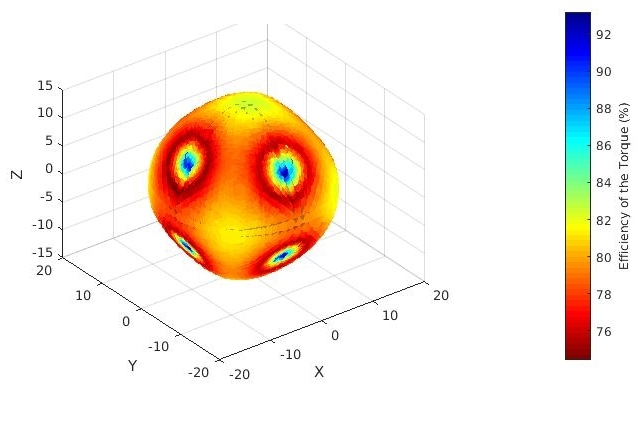
\includegraphics[width=\linewidth]{images/Quad_design_2_tspace.jpg}
    \caption{Attainable torque space.} \label{fig:deisgn1_tspace}
  \end{subfigure}
  \begin{subfigure}[b]{0.52\textwidth}
    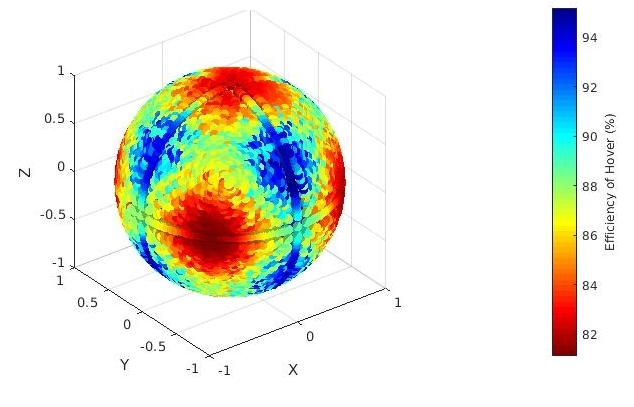
\includegraphics[width=\linewidth]{images/Quad_design_2_hspace.jpg}
    \caption{Hover efficiency in every orientation.} \label{fig:deisgn1_hspace}
  \end{subfigure}}
  \caption{Visual representation of the abilities of Design 1.}
  \label{fig:Quadcopter1_spaces}
\end{figure}
\begin{figure}[!h]
  \resizebox{\textwidth}{!}{\begin{subfigure}[b]{0.55\textwidth}
    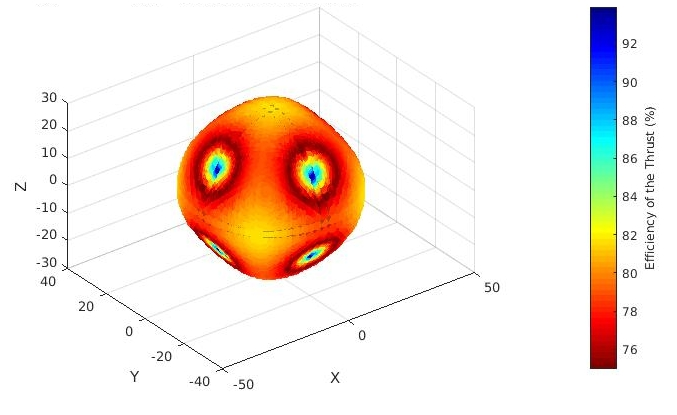
\includegraphics[width=\linewidth]{images/Quad_design_1_fspace.jpg}
    \caption{Attainable force space.} \label{fig:deisgn2_fspace}
  \end{subfigure}
  \hspace*{\fill} % separation between the subfigures
  \begin{subfigure}[b]{0.52\textwidth}
    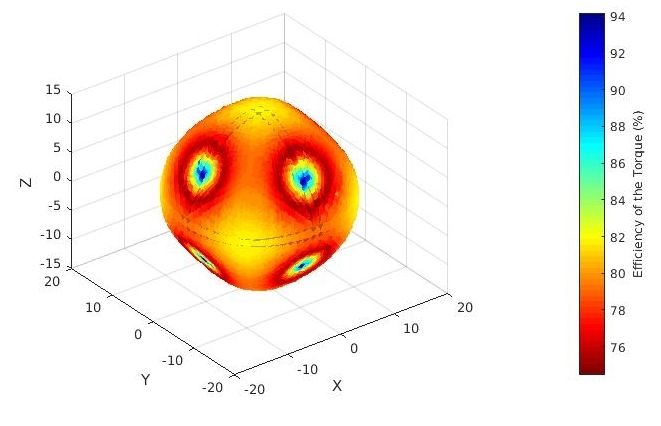
\includegraphics[width=\linewidth]{images/Quad_design_1_tspace.jpg}
    \caption{Attainable torque space.} \label{fig:deisgn2_tspace}
  \end{subfigure}
  \begin{subfigure}[b]{0.5\textwidth}
    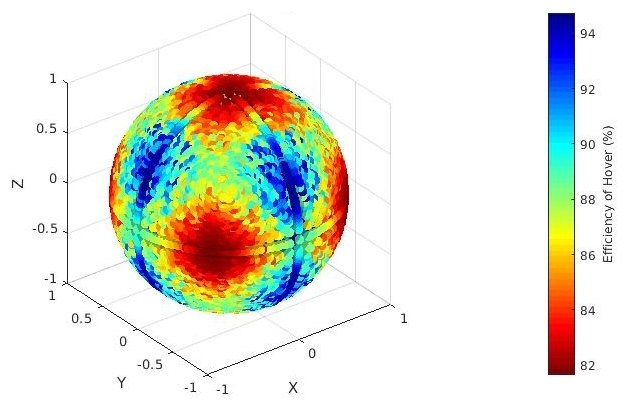
\includegraphics[width=\linewidth]{images/Quad_design_1_hspace.jpg}
    \caption{Hover efficiency in every orientation.} \label{fig:deisgn2_hspace}
  \end{subfigure}}
  \caption{Visual representation of the abilities of Design 2.}
  \label{fig:Quadcopter2_spaces}
\end{figure}
In the following tables, a comparison between the metrics of the optimal designs
and the standard quad-copter is proposed. Due to the tilting ability of the rotors,
the standard design is equally fully-actuated. Even though the force that the standard
quad-copter design can apply in the $Z$ direction is big, the forces that it can
apply on its side and in average are much more limited. We also notice that the
optimal designs proposed by the tool are actually meeting the omni-directionality
criteria stated in \Cref{sec:cost_functions}. Indeed, compared to the standard
design, the minimal forces and torques that the optimal designs can apply are high.
Furthermore, the volumes of the attainable forces and torques are big and shaped
like spheres, which makes the MAVs dynamical properties nearly invariant to their
orientation. Therefore it is not an overstatement to say that they are omni-directional.
\begin{table}[!h]
\begin{center}
 \caption{Force capabilities of the designs.}\vspace{1ex}
 \label{tab:tab_Quad_compare_force}
 \resizebox{\textwidth}{!}{\begin{tabular}{|c|cccccc|}
 \hline
 Design & $F_{min}\ [N]$ & $F_{max}\ [N]$ & $F_{mean}\ [N]$ & $MAD(F)\ [N]$
 & Force space volume $[N^3]$& Force space surface $[N^2]$\\ \hline
  1 & 23.19 & 28.56 & 26.87 & 0.86 & 81'683 & 9'345\\
  2 & 23.23 & 28.37 & 26.87 & 0.86 & 81'710 & 9'326\\
  Standard & 17.37 & 34.74 & 24.43 & 3.43 & 65’673 & 8’865\\
 \hline
 \end{tabular}}
\end{center}
\end{table}
\begin{table}[!h]
\begin{center}
 \caption{Torque capabilities of the designs .}\vspace{1ex}
 \label{tab:tab_Quad_compare_torque}
 \resizebox{\textwidth}{!}{\begin{tabular}{|c|cccccc|}
 \hline
 Design & $M_{min}\ [Nm]$ & $M_{max}\ [Nm]$ & $M_{mean}\ [Nm]$ & $MAD(M)\ [Nm]$
 & Torque space volume $[N^3m^3]$ & Torque space surface $[N^2m^2]$\\ \hline
 1 & 11.62 & 14.32 & 13.47 & 0.43 & 10'298 & 2'355\\
 2 & 11.65 & 14.23 & 13.47 & 0.43 & 10'300 & 2'348\\
 Standard & 8.7 & 17.42 & 12.25 & 1.72 & 8’284 & 2’219\\
 \hline
 \end{tabular}}
\end{center}
\end{table}
\begin{table}[!h]
\begin{center}
 \caption{Hover efficiency of the designs.}\vspace{1ex}
 \label{tab:tab_Quad_compare_hover}
 {\tiny\begin{tabular}{|c|cccc|}
 \hline
  Design & $H_{eff,min}\ [\%]$ & $H_{eff,max}\ [\%]$ & $H_{eff,mean}\ [\%]$
  & $MAD(H_{eff})\ [\%]$\\ \hline
  1 & 81.11 & 95.18 & 87.03 & 2.63\\
  2 & 81.65 & 94.73 & 87.1 & 2.6\\
  Standard & 70.7 & 100 & 82.3 & 6.1\\
 \hline
\end{tabular}}
\end{center}
\end{table}

\subsection{Hexa-copter}
\label{sec:hexa_copter}

Optimal hexa-copter:
\begin{itemize}
  \item $n\ =\ 6$
  \item $\beta_{arm}\ =\ [35.26^{\circ},\  -35.26^{\circ},\  35.26^{\circ},\  -35.26^{\circ},\
                          35.26^{\circ},\  -35.26^{\circ}]$
  \item $\theta_{arm}\ =\ [0^{\circ},\  0^{\circ},\  0^{\circ},\  0^{\circ},\ 0^{\circ},\  0^{\circ}]$
  \item $L\ =\ 0.5\ [m]$
\end{itemize}

Voliro:
\begin{itemize}
  \item $n\ =\ 6$
  \item $\beta_{arm}\ =\ [0^{\circ},\  0^{\circ},\  0^{\circ},\  0^{\circ},\ 0^{\circ},\  0^{\circ}]$
  \item $\theta_{arm}\ =\ [0^{\circ},\  0^{\circ},\  0^{\circ},\  0^{\circ},\ 0^{\circ},\  0^{\circ}]$
  \item $L\ =\ 0.5\ [m]$
\end{itemize}

\begin{figure}[!h]
  \resizebox{\textwidth}{!}{\begin{subfigure}[b]{0.55\textwidth}
    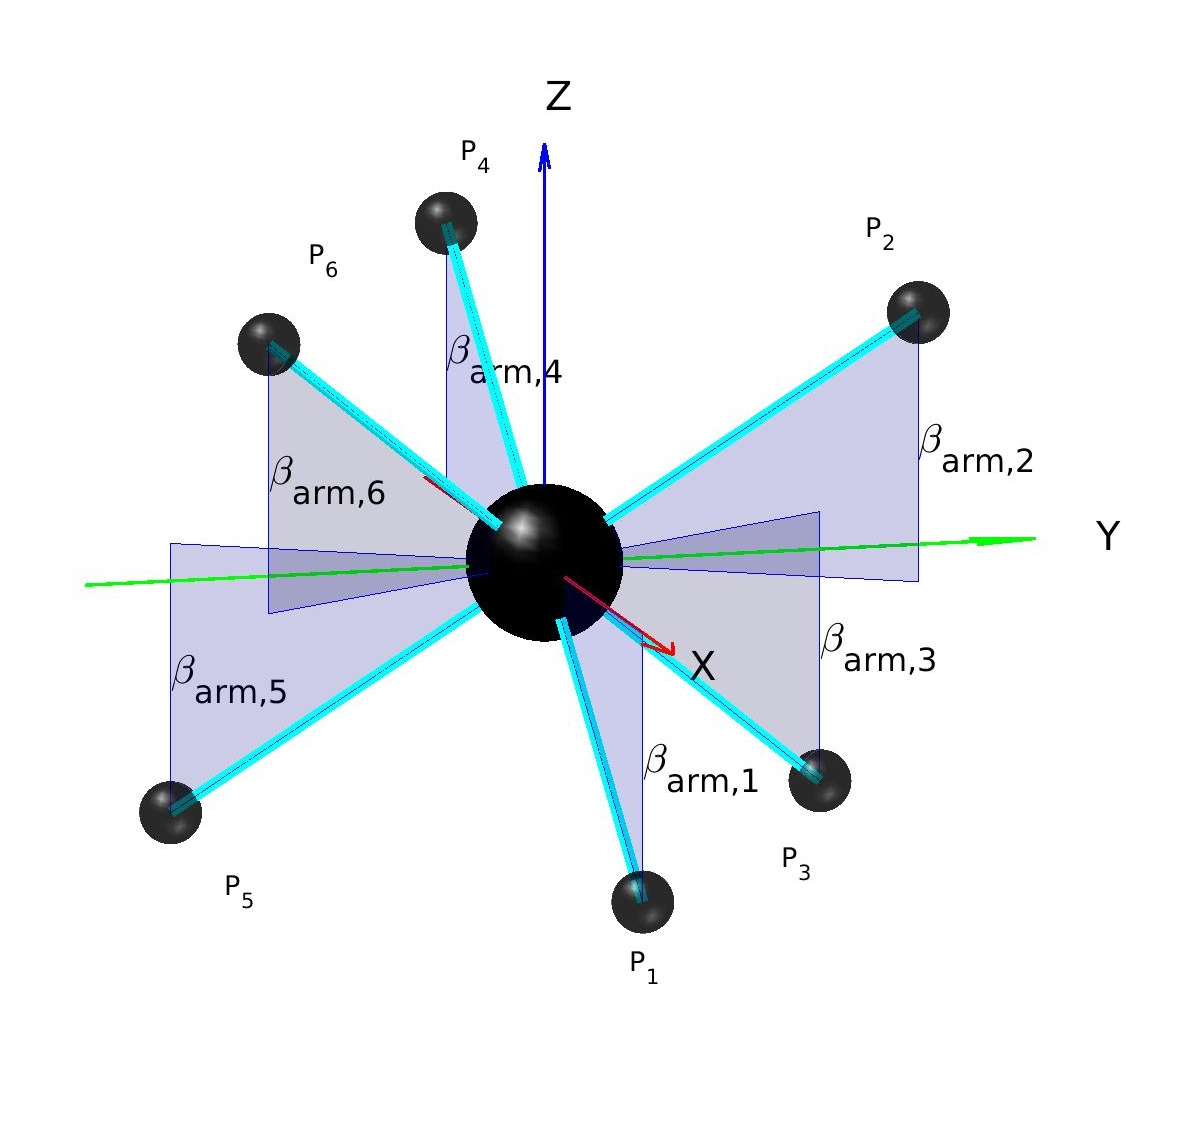
\includegraphics[width=\linewidth]{images/Hexacopter.jpg}
    \caption{Optimal hexa-copter} \label{fig:Hexacopter_resulta}
  \end{subfigure}
  \hspace*{\fill} % separation between the subfigures
  \begin{subfigure}[b]{0.5\textwidth}
    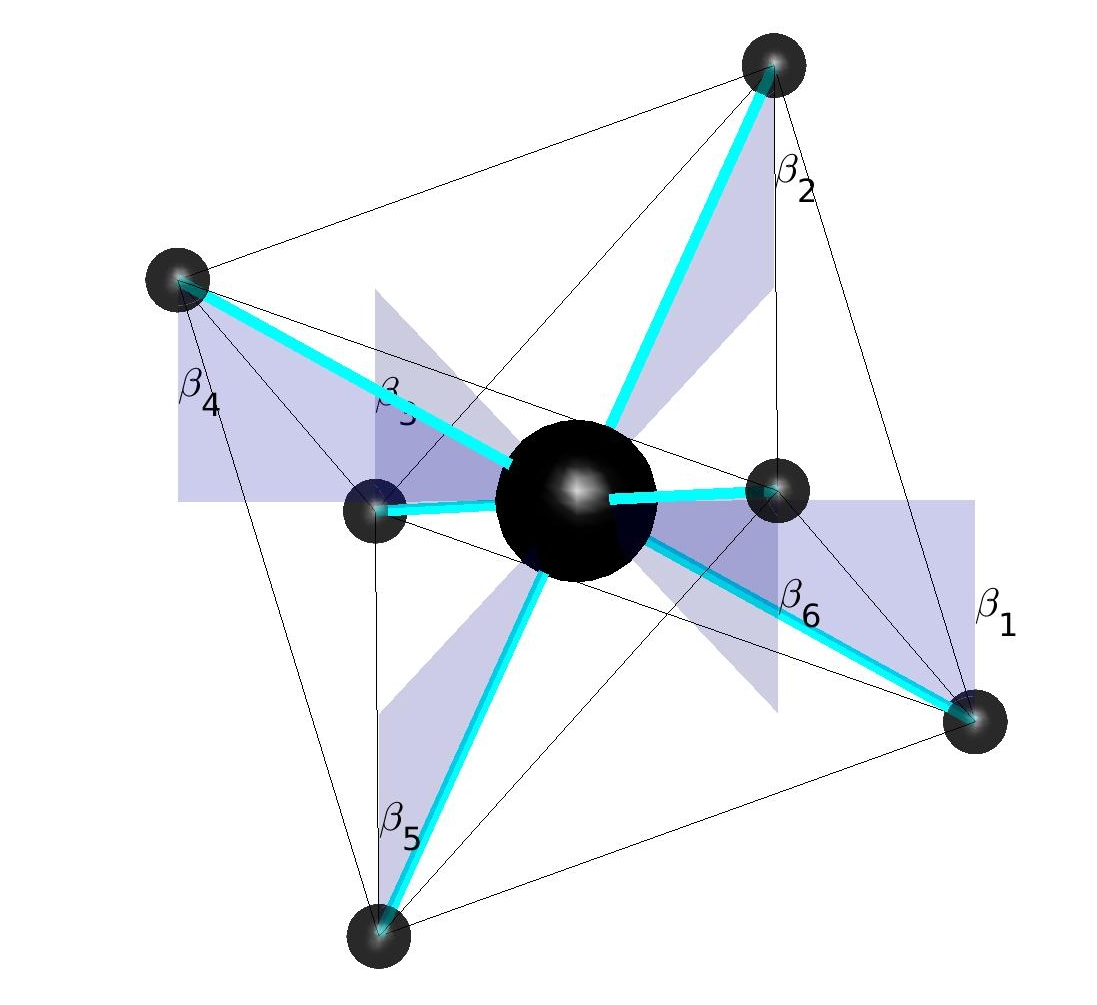
\includegraphics[width=\linewidth]{images/Hexa_octahedron.jpg}
    \caption{Hexa-copter in an octahedron.} \label{fig:Hexacopter_resultb}
  \end{subfigure}
  \hspace*{\fill} % separation between the subfigures
  \begin{subfigure}[b]{0.7\textwidth}
    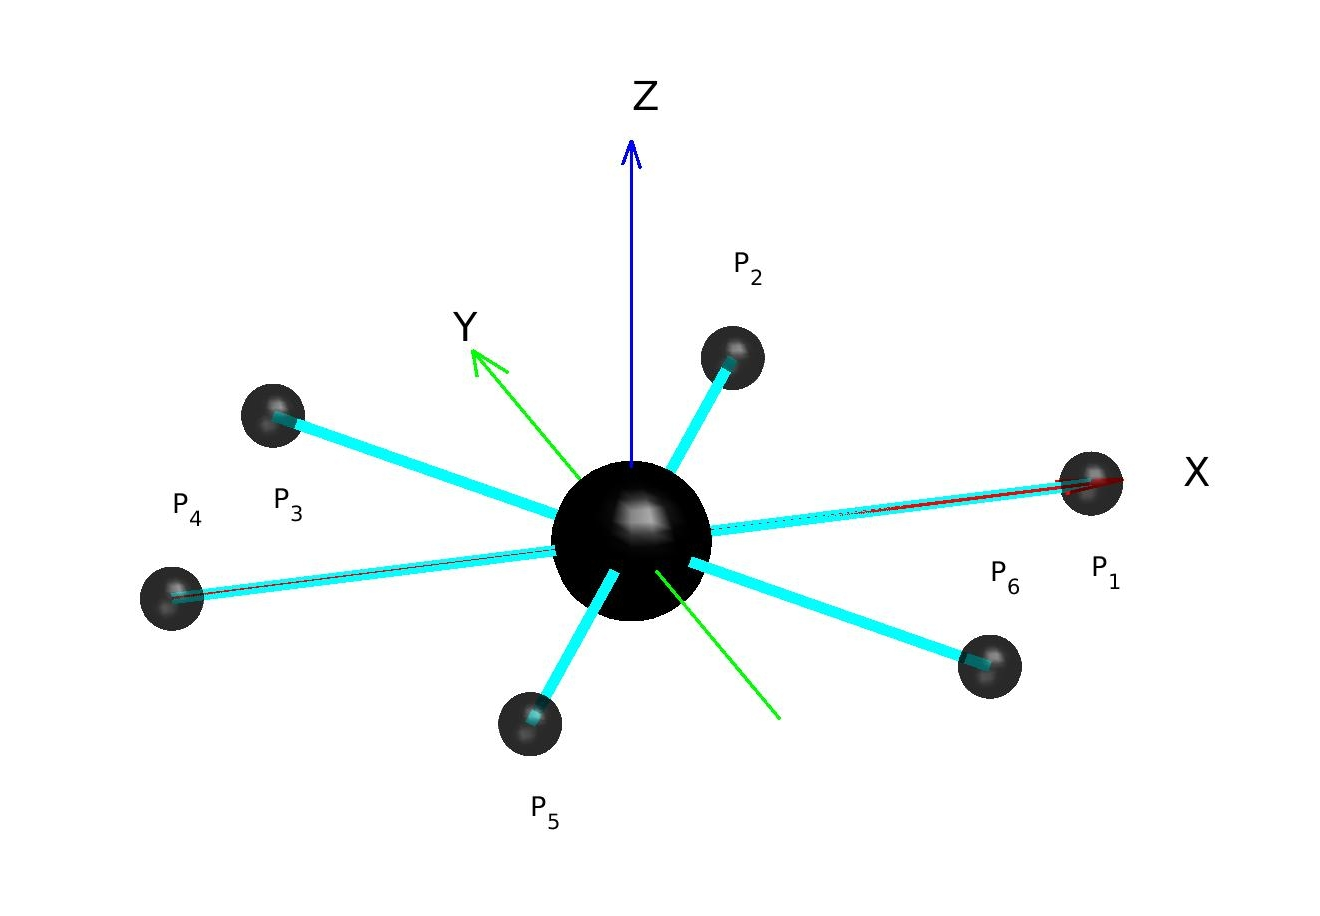
\includegraphics[width=\linewidth]{images/Voliro.jpg}
    \caption{Voliro's design for comparison.} \label{fig:Hexacopter_resultc}
  \end{subfigure}}
  \caption{Schematic of the differnt possible designs for an Hexa-copter.}
  \label{fig:Hexacopter_result}
\end{figure}

\begin{figure}[!h]
  \resizebox{\textwidth}{!}{\begin{subfigure}[b]{0.55\textwidth}
    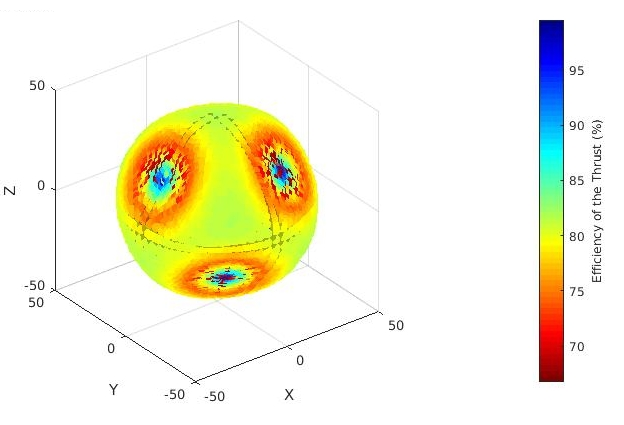
\includegraphics[width=\linewidth]{images/Hexa_fspace.jpg}
    \caption{Attainable force space.} \label{fig:hexa_fspace}
  \end{subfigure}
  \hspace*{\fill} % separation between the subfigures
  \begin{subfigure}[b]{0.5\textwidth}
    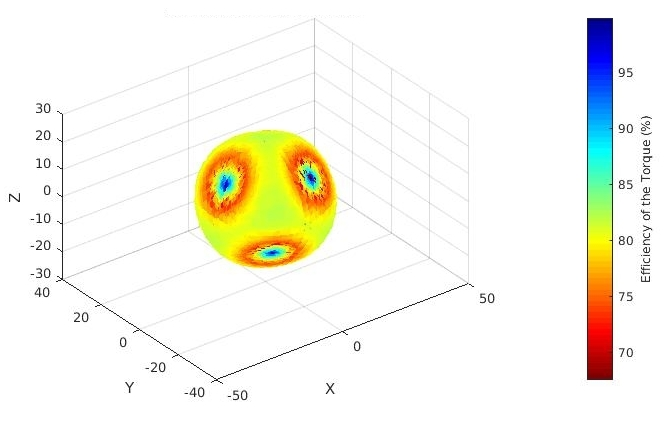
\includegraphics[width=\linewidth]{images/Hexa_tspace.jpg}
    \caption{Attainable torque space.} \label{fig:hexa_tspace}
  \end{subfigure}
  \begin{subfigure}[b]{0.45\textwidth}
    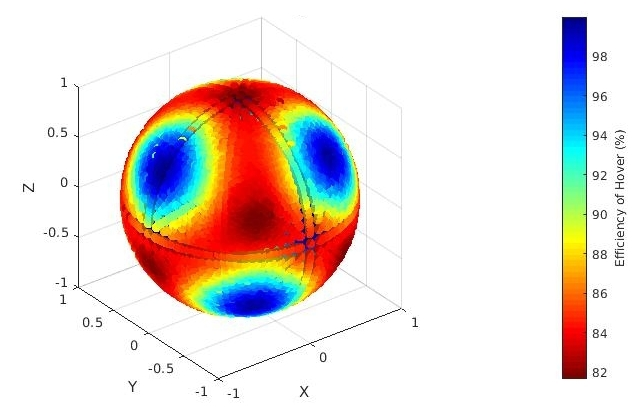
\includegraphics[width=\linewidth]{images/Hexa_hspace.jpg}
    \caption{Hover efficiency in every orientation.} \label{fig:hexa_hspace}
  \end{subfigure}}
  \caption{Representation of the capacities of the optimal hexa-copter.}
  \label{fig:Hexacopter_spaces}
\end{figure}

\begin{figure}[!h]
  \resizebox{\textwidth}{!}{\begin{subfigure}[b]{0.55\textwidth}
    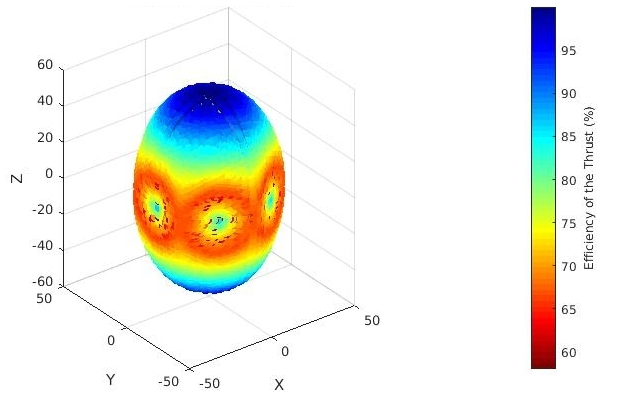
\includegraphics[width=\linewidth]{images/Voliro_fspace.jpg}
    \caption{Attainable force space.} \label{fig:voliro_fspace}
  \end{subfigure}
  \hspace*{\fill} % separation between the subfigures
  \begin{subfigure}[b]{0.5\textwidth}
    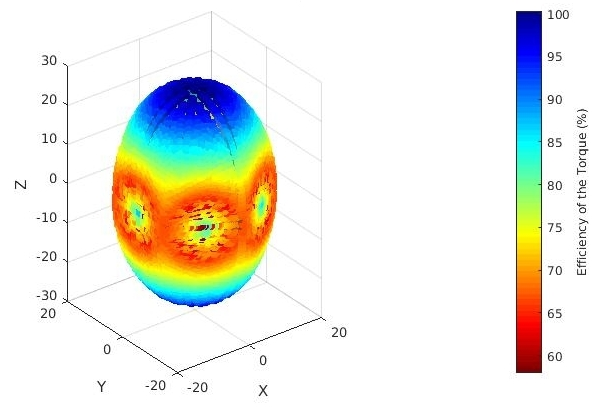
\includegraphics[width=\linewidth]{images/Voliro_tspace.jpg}
    \caption{Attainable torque space.} \label{fig:voliro_tspace}
  \end{subfigure}
  \begin{subfigure}[b]{0.45\textwidth}
    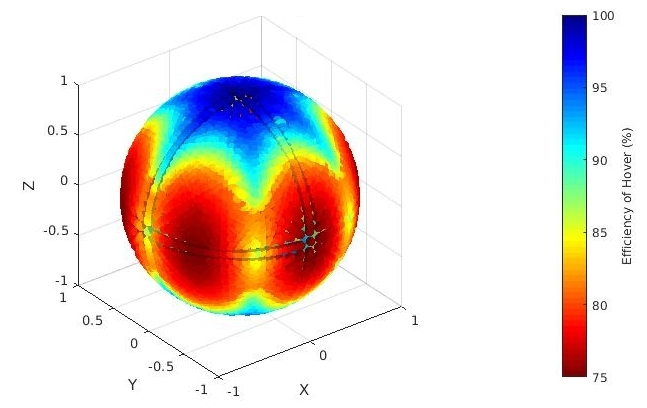
\includegraphics[width=\linewidth]{images/Voliro_hspace.jpg}
    \caption{Hover efficiency in every orientation.} \label{fig:voliro_hspace}
  \end{subfigure}}
  \caption{Representation of the capacities of Voliro.}
  \label{fig:Voliro_spaces}
\end{figure}

\begin{table}[!h]
\begin{center}
 \caption{Comparison between the two designs' force capabilities.}\vspace{1ex}
 \label{tab:tab_Hexa_compare_force}
 \resizebox{\textwidth}{!}{\begin{tabular}{|l|cccccc|}
 \hline
 Design & $F_{min}\ [N]$ & $F_{max}\ [N]$ & $F_{mean}\ [N]$ & $MAD(F)\ [N]$
 & Force space volume $[N^3]$& Force space surface $[N^2]$\\ \hline
 Optimal hexa-copter & 34.74 & 42.55 & 39.52 & 2.21 & 267'010 & 20'922\\
 Voliro & 26.6 & 52.11 & 37.77 & 4.33 & 244'293 & 20'170\\
 \hline
 \end{tabular}}
\end{center}
\end{table}

\begin{table}[!h]
\begin{center}
 \caption{Comparison between the two designs' torque capabilities.}\vspace{1ex}
 \label{tab:tab_Hexa_compare_torque}
 \resizebox{\textwidth}{!}{\begin{tabular}{|l|cccccc|}
 \hline
 Design & $M_{min}\ [Nm]$ & $M_{max}\ [Nm]$ & $M_{mean}\ [Nm]$ & $MAD(M)\ [Nm]$
 & Torque space volume $[N^3m^3]$ & Torque space surface $[N^2m^2]$\\ \hline
 Optimal hexa-copter & 17.42 & 21.34 & 19.82 & 1.1 & 33'687 & 5'230\\
 Voliro & 15.09 & 26.13 & 18.94 & 2.17 & 30'788 & 5'121\\
 \hline
 \end{tabular}}
\end{center}
\end{table}

\begin{table}[!h]
\begin{center}
 \caption{Comparison between two designs' hover capabilities.}\vspace{1ex}
 \label{tab:tab_Hexa_compare_hover}
 \resizebox{\textwidth}{!}{\begin{tabular}{|l|cccc|}
 \hline
  Design & $H_{eff,min}\ [\%]$ & $H_{eff,max}\ [\%]$ & $H_{eff,mean}\ [\%]$
  & $MAD(H_{eff})\ [\%]$\\ \hline
  Optimal hexa-copter & 81.65 & 100 & 88.92 & 4.43\\
  Voliro & 75 & 100 & 84.21 & 5.35\\
 \hline
\end{tabular}}
\end{center}
\end{table}

\subsection{Octa-copter}
\label{sec:octa_copter}

Optimal octa-copter:
\begin{itemize}
  \item $n\ =\ 8$
  \item $\beta_{arm}\ =\ [35.26^{\circ},\  -35.26^{\circ},\  35.26^{\circ},\  -35.26^{\circ},\
                          35.26^{\circ},\  -35.26^{\circ},\ 35.26^{\circ},\  -35.26^{\circ}]$
  \item $\theta_{arm}\ =\ [0^{\circ},\  0^{\circ},\  0^{\circ},\  0^{\circ},\ 0^{\circ},\  0^{\circ},\ 0^{\circ},\  0^{\circ}]$
  \item $L\ =\ 0.5\ [m]$
\end{itemize}

Omnicopter:
\begin{itemize}
  \item $n\ =\ 8$
  \item $\beta_{arm}\ =\ [-35.26^{\circ},\  -35.26^{\circ},\  -35.26^{\circ},\  -35.26^{\circ},\
                          35.26^{\circ},\  35.26^{\circ},\ 35.26^{\circ},\  35.26^{\circ}]$
  \item $\theta_{arm}\ =\ [0^{\circ},\  45^{\circ},\  90^{\circ},\  135^{\circ},\
                          180^{\circ},\  -135^{\circ},\ -90^{\circ},\  -45^{\circ}]$
  \item $L\ =\ 0.5\ [m]$
\end{itemize}

\begin{figure}[!h]
  \resizebox{\textwidth}{!}{\begin{subfigure}[b]{0.6\textwidth}
    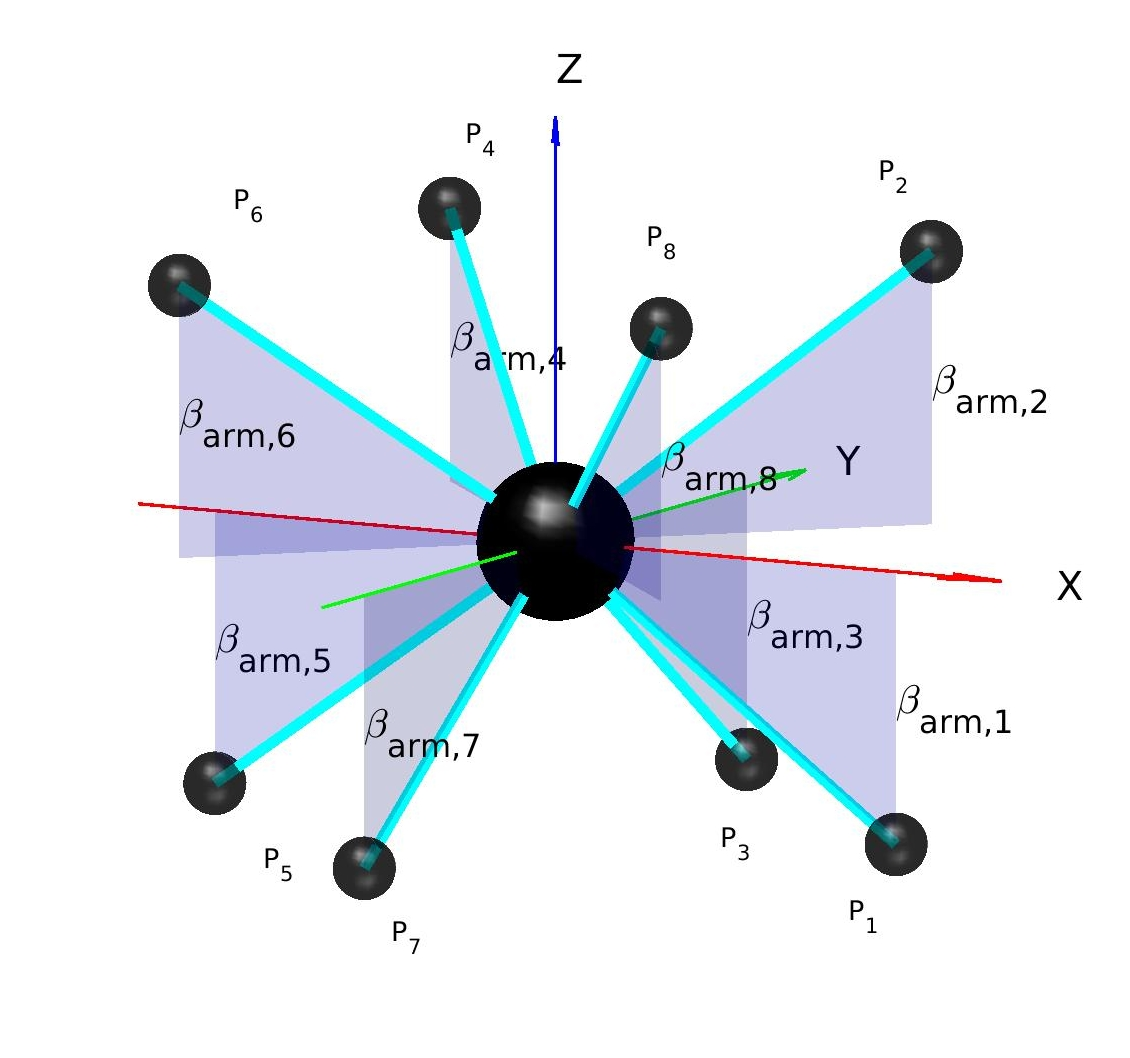
\includegraphics[width=\linewidth]{images/Octacopter.jpg}
    \caption{Optimal hexa-copter} \label{fig:Octacopter_resulta}
  \end{subfigure}
  \hspace*{\fill} % separation between the subfigures
  \begin{subfigure}[b]{0.6\textwidth}
    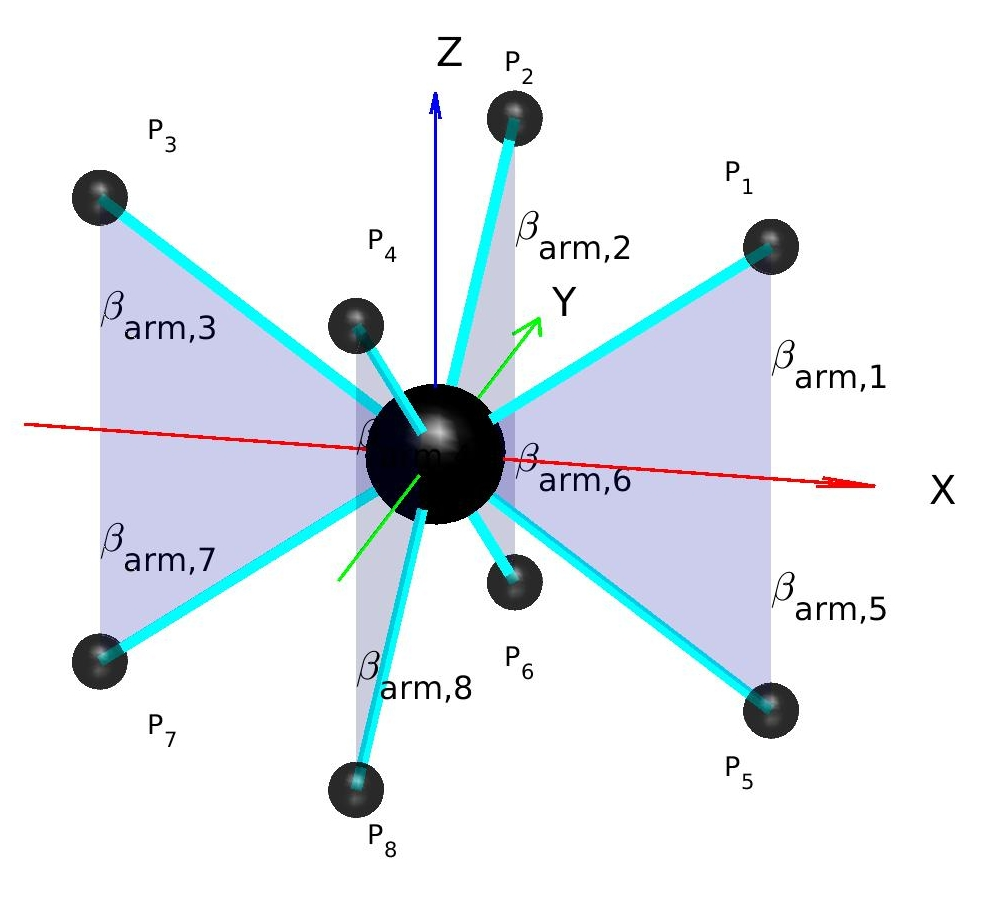
\includegraphics[width=\linewidth]{images/omnicopter.jpg}
    \caption{Omnicopter's design for comparison.} \label{fig:Octacopter_resultb}
  \end{subfigure}
  \hspace*{\fill} % separation between the subfigures
  \begin{subfigure}[b]{0.5\textwidth}
    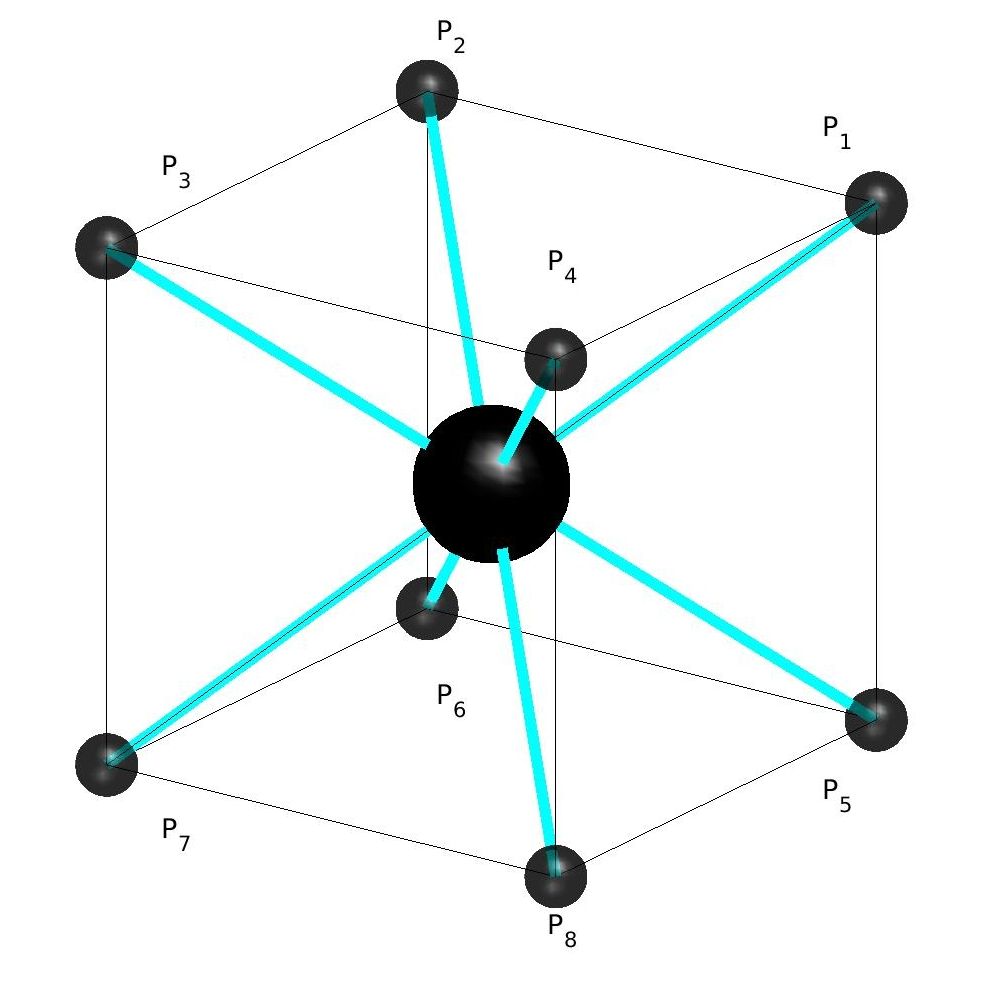
\includegraphics[width=\linewidth]{images/Octa_cube.jpg}
    \caption{Omnicopter in a cube.} \label{fig:Octacopter_resultc}
  \end{subfigure}}
  \caption{Schematic of the differnt possible designs for an Octa-copter.}
  \label{fig:Octacopter_result}
\end{figure}

\begin{figure}[!h]
  \resizebox{\textwidth}{!}{\begin{subfigure}[b]{0.55\textwidth}
    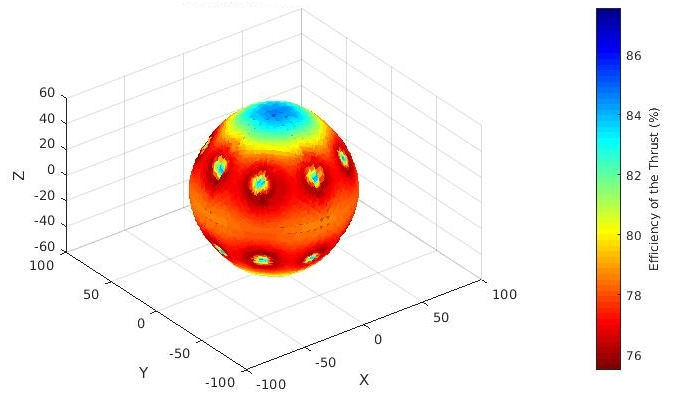
\includegraphics[width=\linewidth]{images/Octa_fspace.jpg}
    \caption{Attainable force space.} \label{fig:Octa_fspace}
  \end{subfigure}
  \hspace*{\fill} % separation between the subfigures
  \begin{subfigure}[b]{0.5\textwidth}
    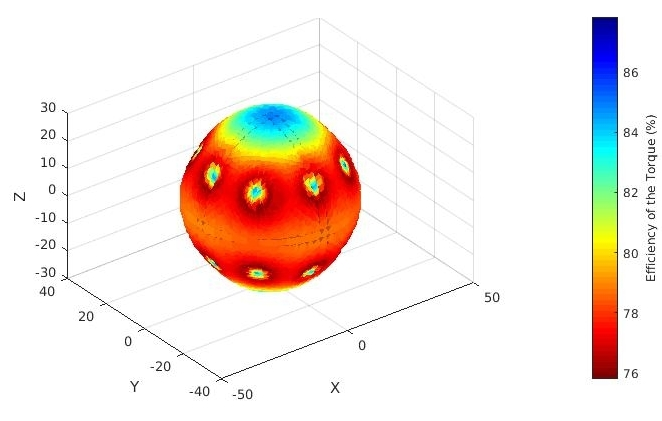
\includegraphics[width=\linewidth]{images/Octa_tspace.jpg}
    \caption{Attainable torque space.} \label{fig:Octa_tspace}
  \end{subfigure}
  \begin{subfigure}[b]{0.45\textwidth}
    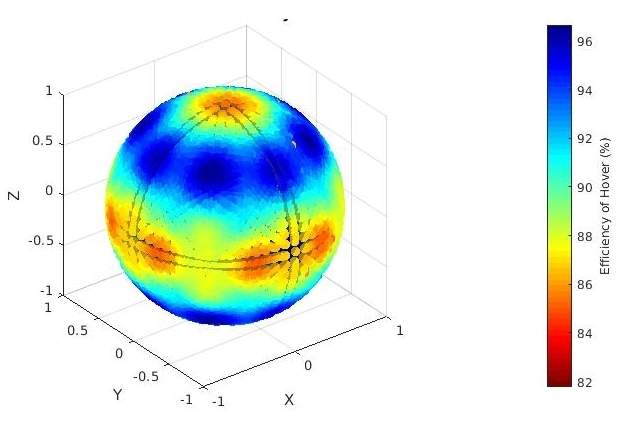
\includegraphics[width=\linewidth]{images/Octa_hspace.jpg}
    \caption{Hover efficiency in every orientation.} \label{fig:Octa_hspace}
  \end{subfigure}}
  \caption{Representation of the capacities of the optimal octa-copter.}
  \label{fig:Octacopter_spaces}
\end{figure}

\begin{figure}[!h]
  \resizebox{\textwidth}{!}{\begin{subfigure}[b]{0.55\textwidth}
    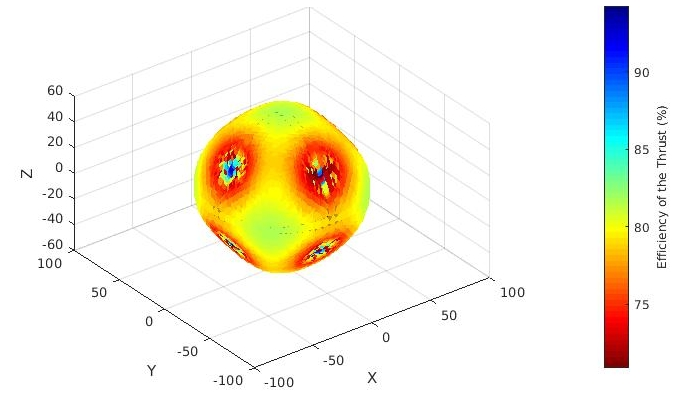
\includegraphics[width=\linewidth]{images/Omnicopter_fspace.jpg}
    \caption{Attainable force space.} \label{fig:Omnicopter_fspace}
  \end{subfigure}
  \hspace*{\fill} % separation between the subfigures
  \begin{subfigure}[b]{0.5\textwidth}
    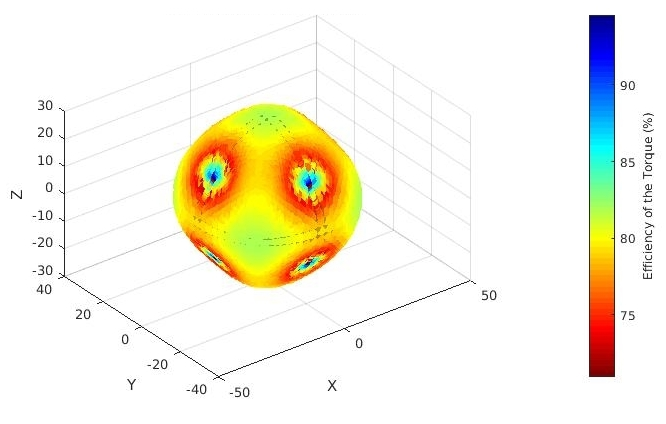
\includegraphics[width=\linewidth]{images/Omnicopter_tspace.jpg}
    \caption{Attainable torque space.} \label{fig:Omnicopter_tspace}
  \end{subfigure}
  \begin{subfigure}[b]{0.45\textwidth}
    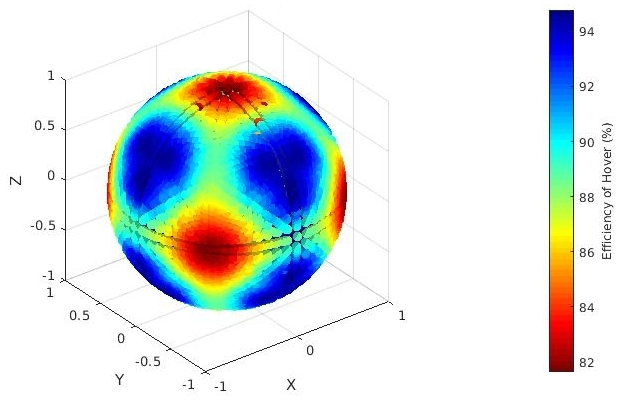
\includegraphics[width=\linewidth]{images/Omnicopter_hspace.jpg}
    \caption{Hover efficiency in every orientation.} \label{fig:Omnicopter_hspace}
  \end{subfigure}}
  \caption{Representation of the capacities of Omnicopter.}
  \label{fig:Omnicopter_spaces}
\end{figure}

\begin{table}[!h]
\begin{center}
 \caption{Comparison between the two designs' force capabilities.}\vspace{1ex}
 \label{tab:tab_Octa_compare_force}
 \resizebox{\textwidth}{!}{\begin{tabular}{|l|cccccc|}
 \hline
 Design & $F_{min}\ [N]$ & $F_{max}\ [N]$ & $F_{mean}\ [N]$ & $MAD(F)\ [N]$
 & Force space volume $[N^3]$& Force space surface $[N^2]$\\ \hline
 Optimal octa-copter & 44.7 & 58.78 & 53.95 & 0.94 & 669'339 & 37'625\\
 Omnicopter & 46.46 & 56.73 & 53.75 & 1.72 & 653'736 & 37'263\\
 \hline
 \end{tabular}}
\end{center}
\end{table}

\begin{table}[!h]
\begin{center}
 \caption{Comparison between the two designs' torque capabilities.}\vspace{1ex}
 \label{tab:tab_Octa_compare_torque}
 \resizebox{\textwidth}{!}{\begin{tabular}{|l|cccccc|}
 \hline
 Design & $M_{min}\ [Nm]$ & $M_{max}\ [Nm]$ & $M_{mean}\ [Nm]$ & $MAD(M)\ [Nm]$
 & Torque space volume $[N^3m^3]$ & Torque space surface $[N^2m^2]$\\ \hline
 Optimal octa-copter & 22.4 & 29.48 & 27 & 0.47 & 84'417 & 9'463\\
 Omnicopter & 23.3 & 28.45 & 26.95 & 0.86 & 82'446 & 9'374\\
 \hline
 \end{tabular}}
\end{center}
\end{table}

\begin{table}[!h]
\begin{center}
 \caption{Comparison between two designs' hover capabilities.}\vspace{1ex}
 \label{tab:tab_Octa_compare_hover}
 \resizebox{\textwidth}{!}{\begin{tabular}{|l|cccc|}
 \hline
  Design & $H_{eff,min}\ [\%]$ & $H_{eff,max}\ [\%]$ & $H_{eff,mean}\ [\%]$
  & $MAD(H_{eff})\ [\%]$\\ \hline
  Optimal octa-copter & 81.78 & 96.65 & 91.42 & 2.7\\
  Omnicopter & 81.64 & 94.77 & 89.36 & 2.82\\
 \hline
\end{tabular}}
\end{center}
\end{table}

\section{Odd Designs}
\label{sec:odd_designs}

\subsection{Tri-copter}
\label{sec:tri_copter}
Optimal tri-copter:
\begin{itemize}
  \item $n\ =\ 3$
  \item $\beta_{arm}\ =\ [35.26^{\circ},\  35.26^{\circ},\  35.26^{\circ}]$
  \item $\theta_{arm}\ =\ [0^{\circ},\  0^{\circ},\  0^{\circ}]$
  \item $L\ =\ 0.5\ [m]$
\end{itemize}

\begin{figure}[!h]
  \resizebox{\textwidth}{!}{
  \begin{subfigure}[b]{0.4\textwidth}
    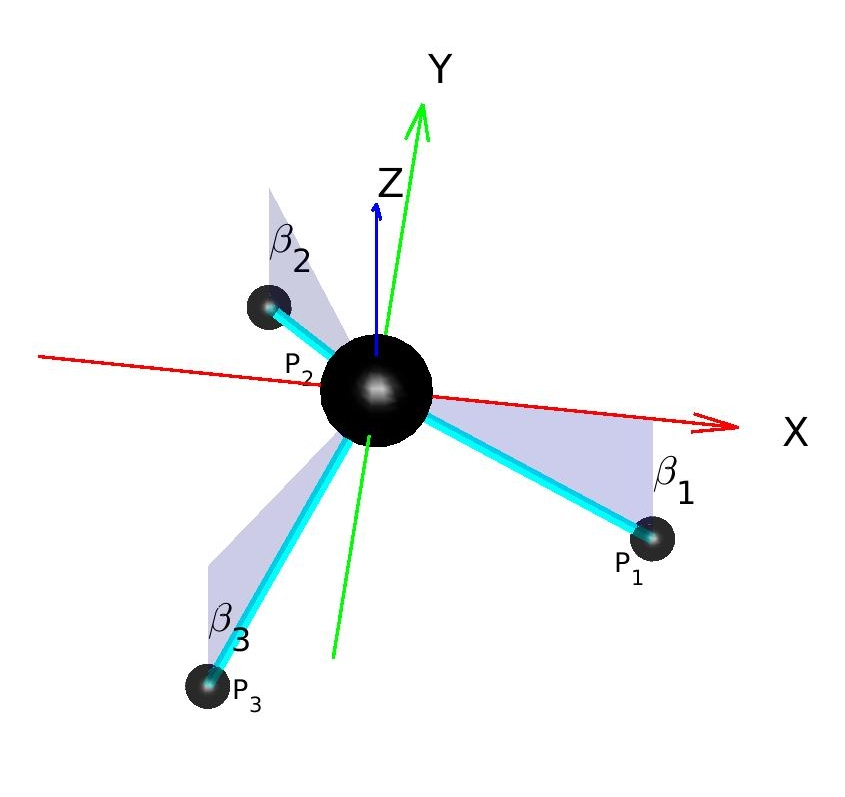
\includegraphics[width=\linewidth]{images/Tricopter.jpg}
    \caption{Design representation.} \label{fig:Tricopter_visual}
  \end{subfigure}
  \hspace*{\fill} % separation between the subfigures
  \begin{subfigure}[b]{0.4\textwidth}
    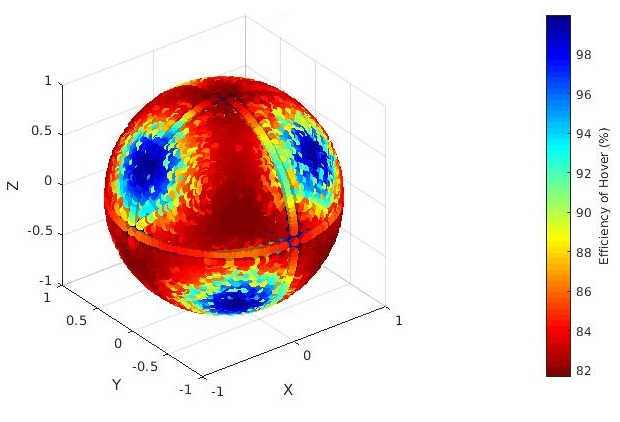
\includegraphics[width=\linewidth]{images/Tri_hspace.jpg}
    \caption{Hover efficiency space.} \label{fig:Tricopter_hspace}
  \end{subfigure}
  }
  \hspace*{\fill} % separation between the subfigures
  \resizebox{\textwidth}{!}{\begin{subfigure}[b]{0.45\textwidth}
    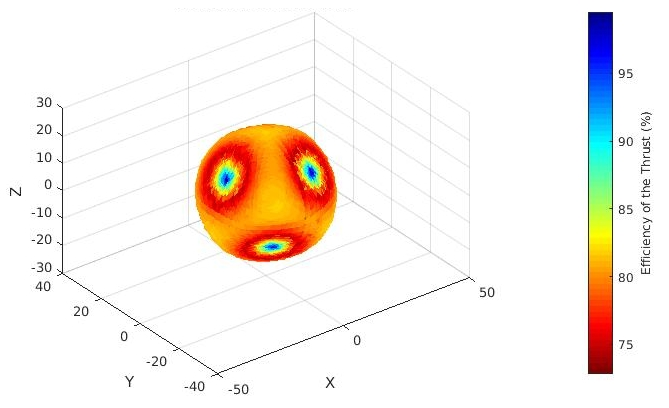
\includegraphics[width=\linewidth]{images/Tri_fspace.jpg}
    \caption{Force space.} \label{fig:Tricopter_fspace}
  \end{subfigure}
  \hspace*{\fill} % separation between the subfigures
  \begin{subfigure}[b]{0.4\textwidth}
    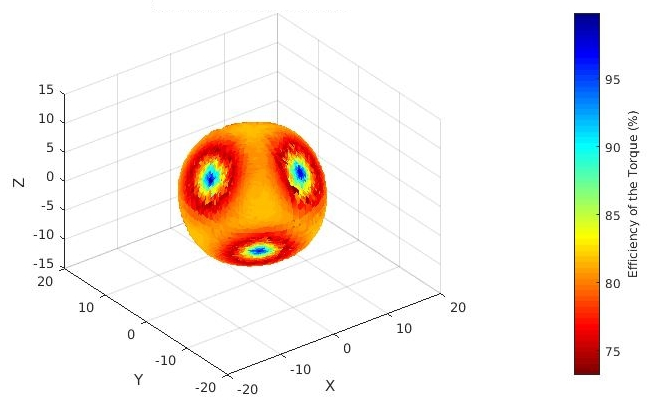
\includegraphics[width=\linewidth]{images/Tri_tspace.jpg}
    \caption{Torque space.} \label{fig:Tricopter_tspace}
  \end{subfigure}}
  \caption{Visual representation of the optimal tri-copter capabilities.}
  \label{fig:Tricopter_result}
\end{figure}

\subsection{Penta-copter}
\label{sec:penta_copter}
Optimal penta-copter:
\begin{itemize}
  \item $n\ =\ 5$
  \item $\beta_{arm}\ =\ [35.26^{\circ},\  35.26^{\circ},\  35.26^{\circ},\  35.26^{\circ},\   35.26^{\circ}]$
  \item $\theta_{arm}\ =\ [0^{\circ},\  0^{\circ},\  0^{\circ},\  0^{\circ},\  0^{\circ}]$
  \item $L\ =\ 0.5\ [m]$
\end{itemize}

Standard penta-copter:
\begin{itemize}
  \item $n\ =\ 5$
  \item $\beta_{arm}\ =\ [0^{\circ},\  0^{\circ},\  0^{\circ},\  0^{\circ},\  0^{\circ}]$
  \item $\theta_{arm}\ =\ [0^{\circ},\  0^{\circ},\  0^{\circ},\  0^{\circ},\  0^{\circ}]$
  \item $L\ =\ 0.5\ [m]$
\end{itemize}
\begin{figure}[!h]
  \begin{subfigure}[b]{0.4\textwidth}
    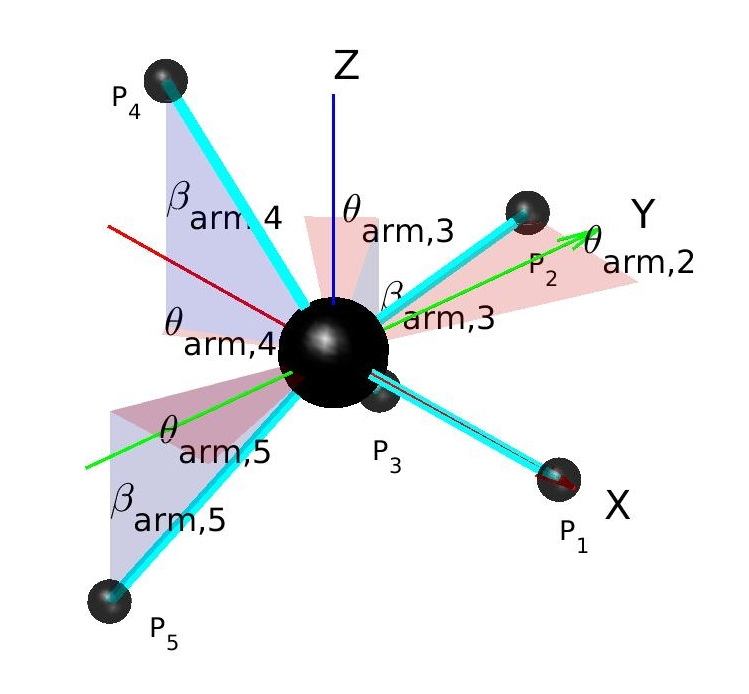
\includegraphics[width=\linewidth]{images/Pentacopter_odd.jpg}
    \caption{Optimal penta-copter.} \label{fig:Pentacopter_odd}
  \end{subfigure}
  \hspace*{\fill} % separation between the subfigures
  \begin{subfigure}[b]{0.5\textwidth}
    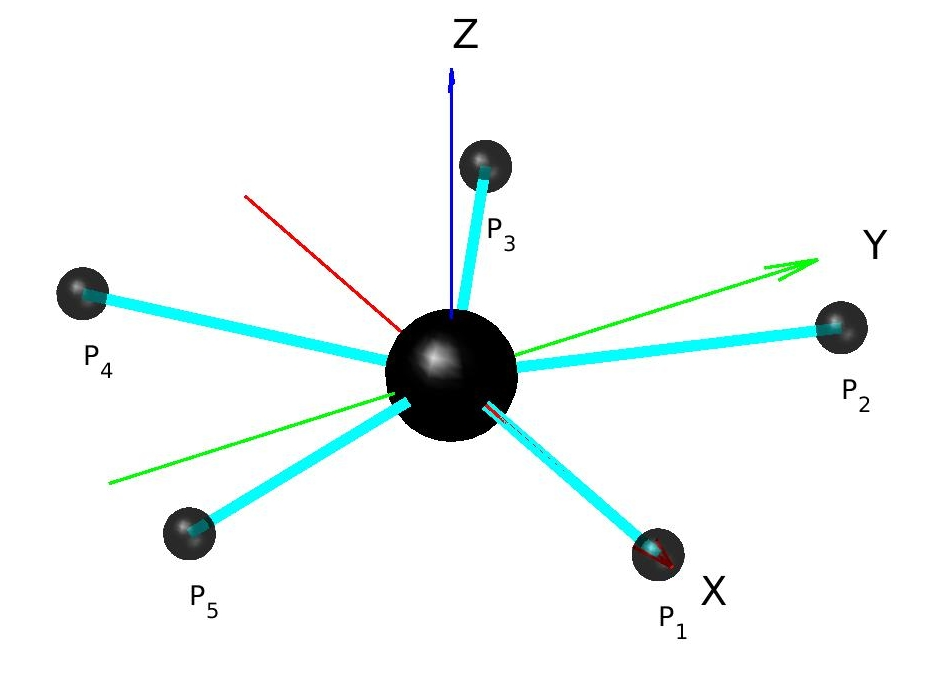
\includegraphics[width=\linewidth]{images/Pentacopter_standard.jpg}
    \caption{Penta-copter standard.} \label{fig:Pentacopter_standard}
  \end{subfigure}
  \caption{Schematic of different possible designs for a Penta-copter.}
  \label{fig:Pentacopter_result}
\end{figure}

\begin{table}[!h]
\begin{center}
 \caption{Comparison between the two designs' force capabilities.}\vspace{1ex}
 \label{tab:tab_Penta_compare_force}
 \resizebox{\textwidth}{!}{\begin{tabular}{|l|cccccc|}
 \hline
 Design & $F_{min}\ [N]$ & $F_{max}\ [N]$ & $F_{mean}\ [N]$ & $MAD(F)\ [N]$
 & Force space volume $[N^3]$& Force space surface $[N^2]$\\ \hline
 Optimal & 26.03 & 36.22 & 33.69 & 1.39 & 160'333 & 14'626\\
 Standard & 26.24 & 43.42 & 31.93 & 3.25 & 146'006 & 14'137\\
 \hline
 \end{tabular}}
\end{center}
\end{table}

\begin{table}[!h]
\begin{center}
 \caption{Comparison between the two designs' torque capabilities.}\vspace{1ex}
 \label{tab:tab_Penta_compare_torque}
 \resizebox{\textwidth}{!}{\begin{tabular}{|l|cccccc|}
 \hline
 Design & $M_{min}\ [Nm]$ & $M_{max}\ [Nm]$ & $M_{mean}\ [Nm]$ & $MAD(M)\ [Nm]$
 & Torque space volume $[N^3m^3]$ & Torque space surface $[N^2m^2]$\\ \hline
 Optimal & 12.85 & 18.2 & 16.93 & 0.7 & 20'358 & 3'741\\
 Standard & 10.9 & 21.8 & 16 & 1.63 & 18'409 & 3'580\\
 \hline
 \end{tabular}}
\end{center}
\end{table}

\begin{table}[!h]
\begin{center}
 \caption{Comparison between two designs' hover capabilities.}\vspace{1ex}
 \label{tab:tab_Penta_compare_hover}
 \resizebox{\textwidth}{!}{\begin{tabular}{|l|cccc|}
 \hline
  Design & $H_{eff,min}\ [\%]$ & $H_{eff,max}\ [\%]$ & $H_{eff,mean}\ [\%]$
  & $MAD(H_{eff})\ [\%]$\\ \hline
  Optimal & 80.33 & 99.4 & 90.96 & 3\\
  Standard & 77.25 & 100 & 84.38 & 5.2\\
 \hline
\end{tabular}}
\end{center}
\end{table}

\begin{figure}[!h]
  \resizebox{\textwidth}{!}{\begin{subfigure}[b]{0.55\textwidth}
    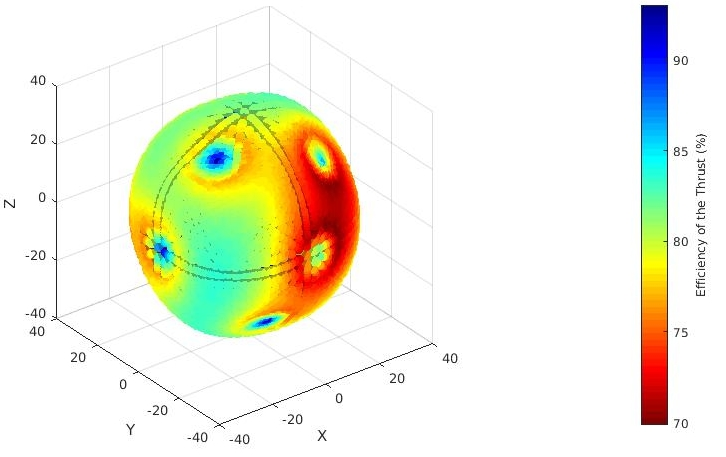
\includegraphics[width=\linewidth]{images/Penta_fspace.jpg}
    \caption{Attainable force space.} \label{fig:penta_fspace}
  \end{subfigure}
  \hspace*{\fill} % separation between the subfigures
  \begin{subfigure}[b]{0.5\textwidth}
    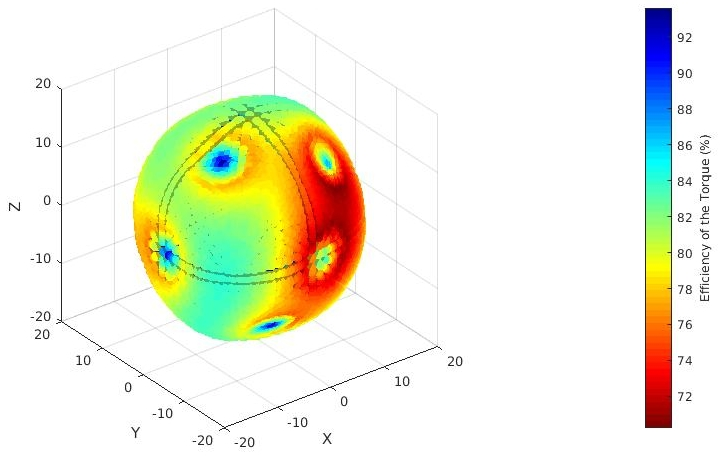
\includegraphics[width=\linewidth]{images/Penta_tspace.jpg}
    \caption{Attainable torque space.} \label{fig:penta_tspace}
  \end{subfigure}
  \begin{subfigure}[b]{0.45\textwidth}
    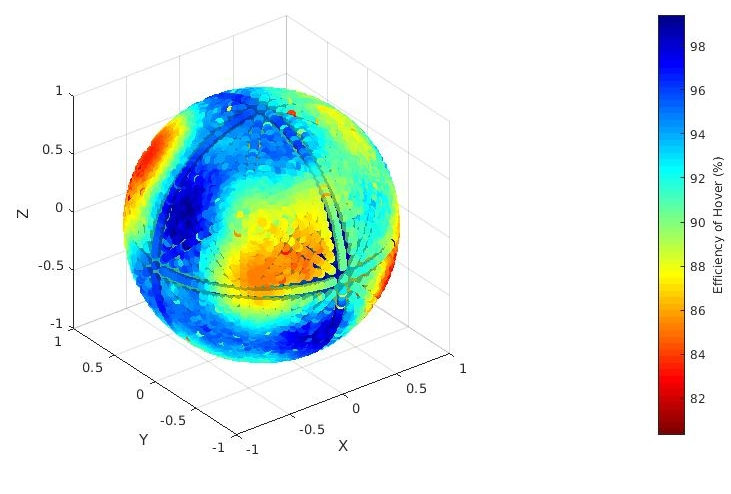
\includegraphics[width=\linewidth]{images/Penta_hspace.jpg}
    \caption{Hover efficiency in every orientation.} \label{fig:penta_hspace}
  \end{subfigure}}
  \caption{Representation of the capacities of the optimal penta-copter.}
  \label{fig:Pentacopter_spaces}
\end{figure}

\begin{figure}[!h]
  \resizebox{\textwidth}{!}{\begin{subfigure}[b]{0.55\textwidth}
    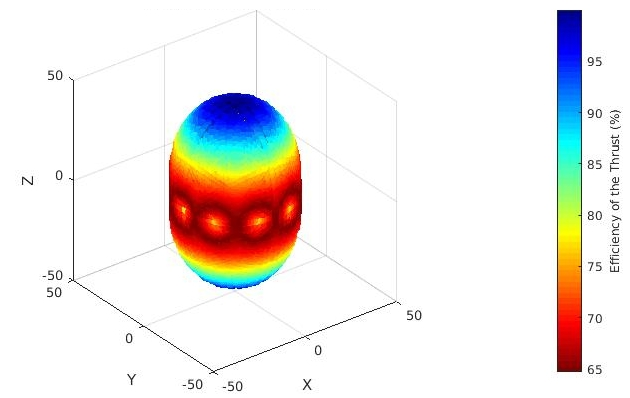
\includegraphics[width=\linewidth]{images/Penta_standard_fspace.jpg}
    \caption{Attainable force space.} \label{fig:penta_standard_fspace}
  \end{subfigure}
  \hspace*{\fill} % separation between the subfigures
  \begin{subfigure}[b]{0.5\textwidth}
    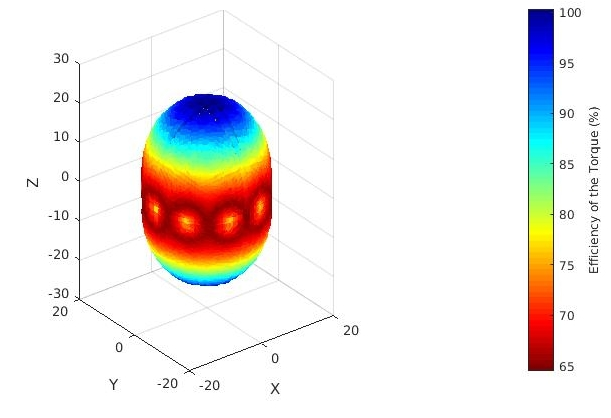
\includegraphics[width=\linewidth]{images/Penta_standard_tspace.jpg}
    \caption{Attainable torque space.} \label{fig:penta_standard_tspace}
  \end{subfigure}
  \begin{subfigure}[b]{0.45\textwidth}
    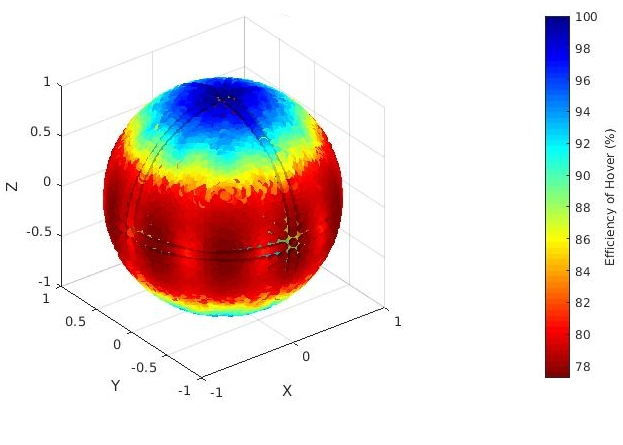
\includegraphics[width=\linewidth]{images/Penta_standard_hspace.jpg}
    \caption{Hover efficiency in every orientation.} \label{fig:penta_standard_hspace}
  \end{subfigure}}
  \caption{Representation of the capacities of the standard penta-copter.}
  \label{fig:penta_standard_spaces}
\end{figure}

\subsection{Hepta-copter}
\label{sec:hepta_copter}
Optimal hepta-copter:
\begin{itemize}
  \item $n\ =\ 7$
  \item $\beta_{arm}\ =\ [35.26^{\circ},\  35.26^{\circ},\  35.26^{\circ},\  35.26^{\circ},\
                          35.26^{\circ},\  35.26^{\circ},\  35.26^{\circ}]$
  \item $\theta_{arm}\ =\ [0^{\circ},\  0^{\circ},\  0^{\circ},\  0^{\circ},\  0^{\circ},\
                            0^{\circ},\  0^{\circ}]$
  \item $L\ =\ 0.5\ [m]$
\end{itemize}

\begin{figure}[!h]
  \begin{center}
    \resizebox{\textwidth}{!}{\begin{subfigure}[b]{0.4\textwidth}
      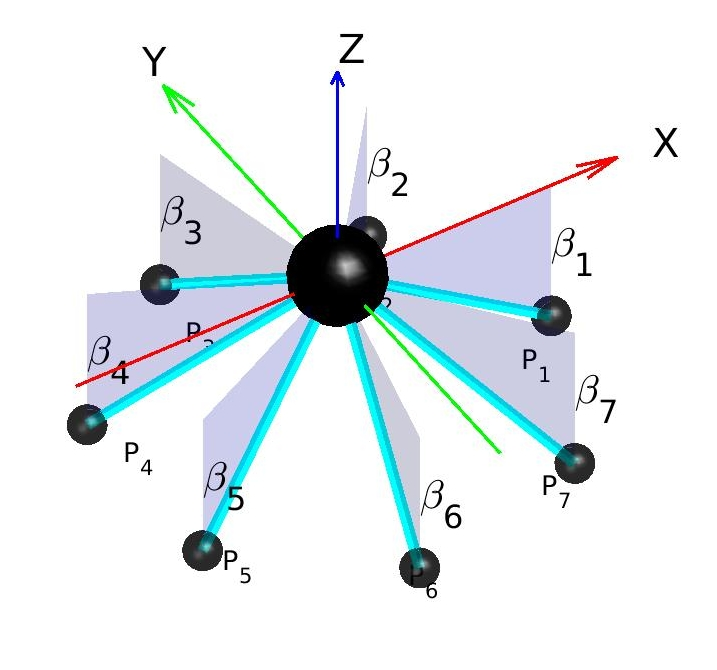
\includegraphics[width=\linewidth]{images/Heptacopter.jpg}
      \caption{Hover efficiency space.} \label{fig:Heptacopter_hspace}
    \end{subfigure}
    \hspace*{\fill} % separation between the subfigures
    \begin{subfigure}[b]{0.45\textwidth}
      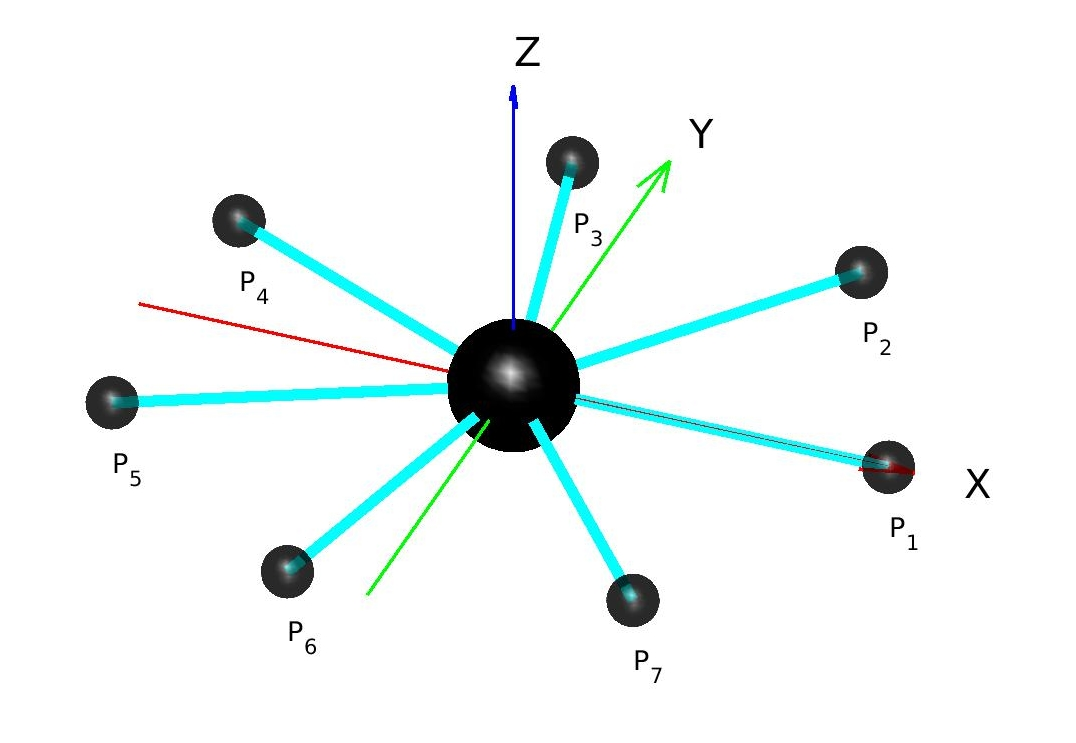
\includegraphics[width=\linewidth]{images/Heptacopter_standard.jpg}
      \caption{Hover efficiency space.} \label{fig:Heptacopter_hspace}
    \end{subfigure}}
    \resizebox{\textwidth}{!}{\begin{subfigure}[b]{0.5\textwidth}
      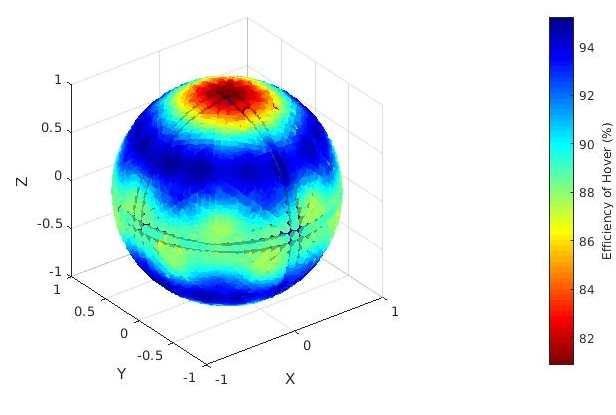
\includegraphics[width=\linewidth]{images/Hepta_opt_hspace.jpg}
      \caption{Optimal design hover efficiency space.} \label{fig:Hepta_opt_hspace}
    \end{subfigure}
    \hspace*{\fill} % separation between the subfigures
    \begin{subfigure}[b]{0.5\textwidth}
      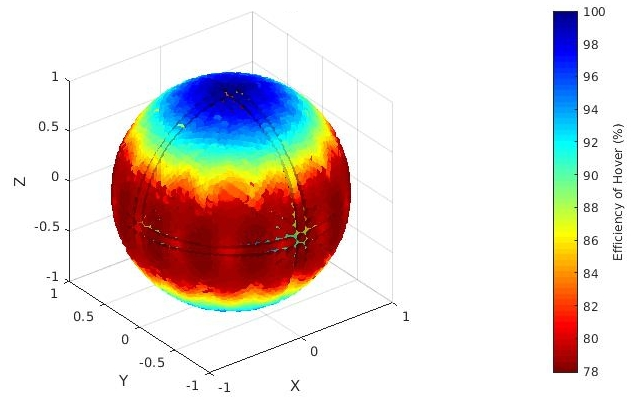
\includegraphics[width=\linewidth]{images/Hepta_hspace.jpg}
      \caption{Standard design hover efficiency space.} \label{fig:Hepta_hspace}
    \end{subfigure}}
    \caption{Visual representation of the optimal Hepta-copter capabilities.}
    \label{fig:Heptacopter_result}
  \end{center}
\end{figure}

\section{Comparison of Different Designs}
\label{sec:comparison}
\begin{figure}[!h]
  \resizebox{\textwidth}{!}{\begin{subfigure}[b]{0.5\textwidth}
    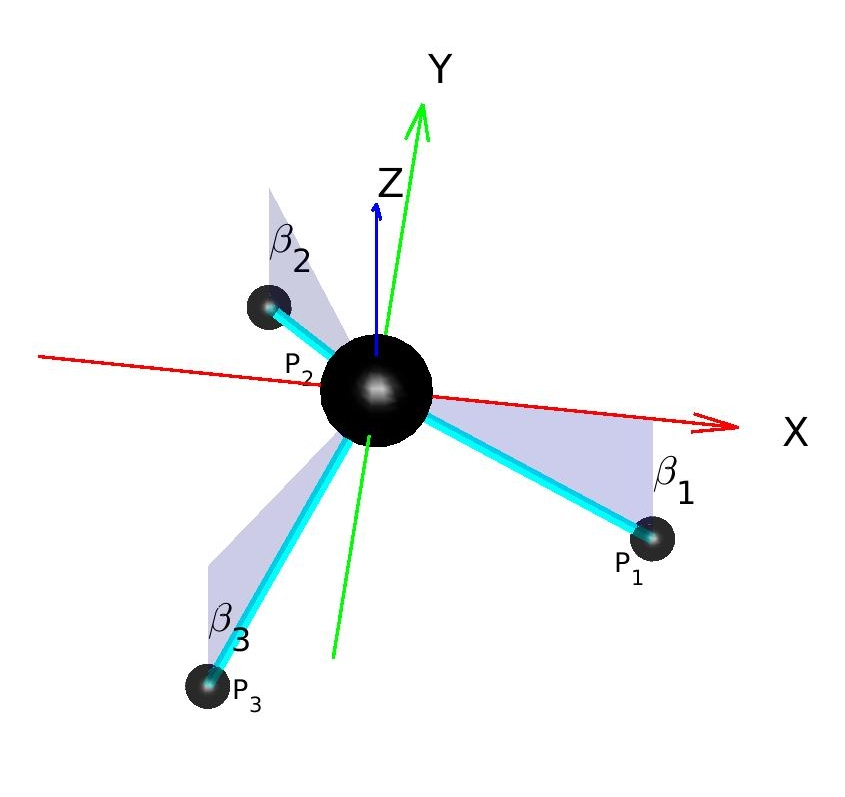
\includegraphics[width=\linewidth]{images/Tricopter.jpg}
    \caption{Tri-copter.} \label{fig:comp_tri}
  \end{subfigure}
  \hspace*{\fill} % separation between the subfigures
  \begin{subfigure}[b]{0.5\textwidth}
    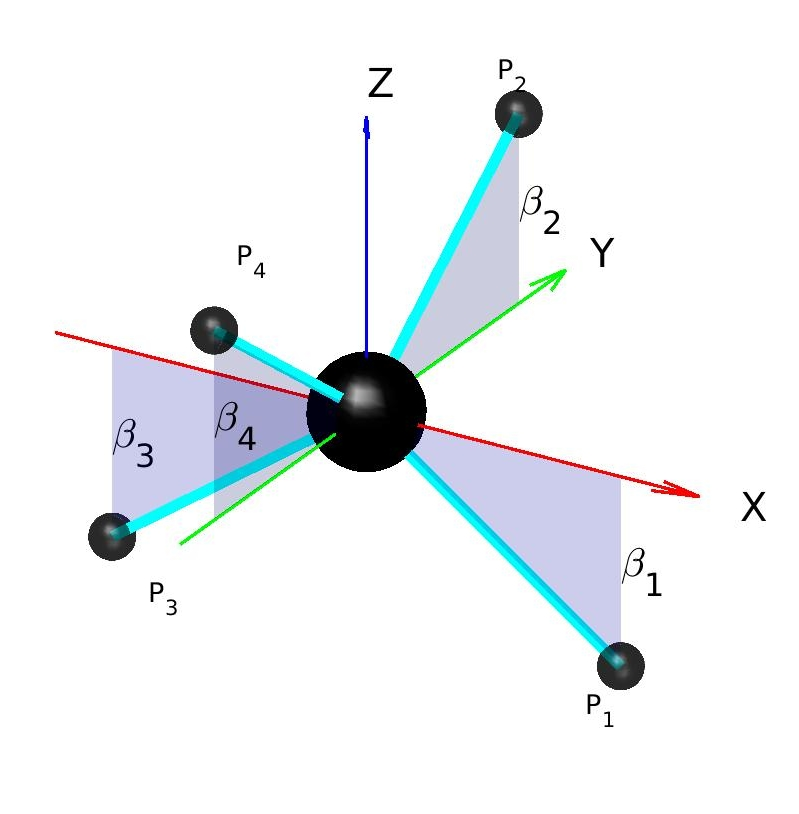
\includegraphics[width=\linewidth]{images/Quadcopter.jpg}
    \caption{Quad-copter.} \label{fig:comp_quad}
  \end{subfigure}
  \begin{subfigure}[b]{0.5\textwidth}
    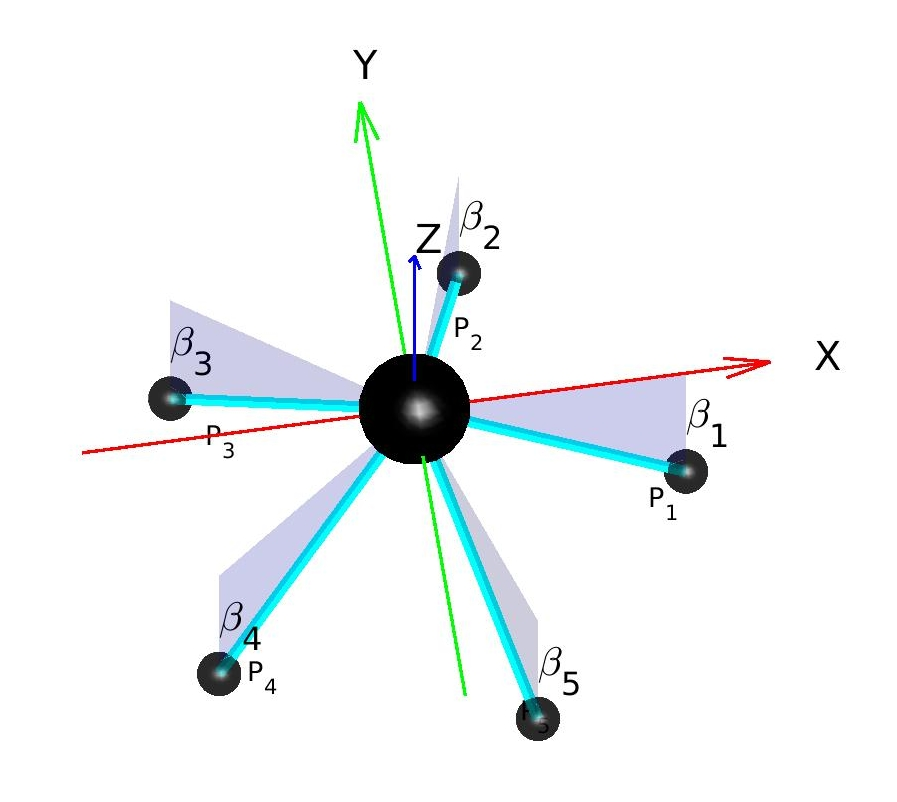
\includegraphics[width=\linewidth]{images/Pentacopter.jpg}
    \caption{Penta-copter.} \label{fig:comp_penta}
  \end{subfigure}}
  \resizebox{\textwidth}{!}{\begin{subfigure}[b]{0.5\textwidth}
    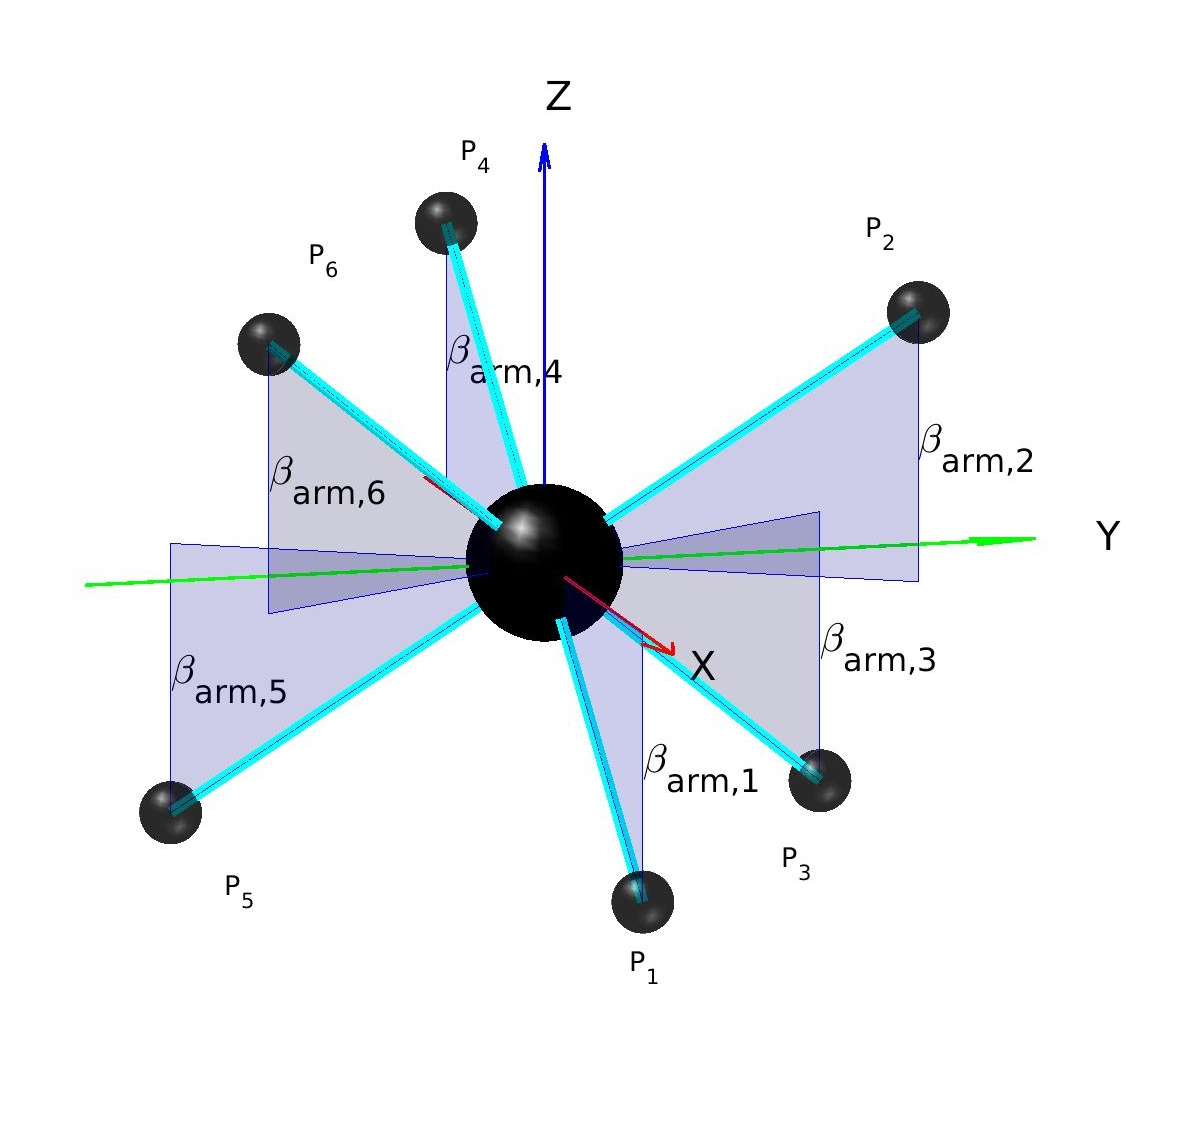
\includegraphics[width=\linewidth]{images/Hexacopter.jpg}
    \caption{Hexa-copter.} \label{fig:comp_hexa}
  \end{subfigure}
  \hspace*{\fill} % separation between the subfigures
  \begin{subfigure}[b]{0.5\textwidth}
    \includegraphics[width=\linewidth]{images/Heptacopter.jpg}
    \caption{Hepta-copter.} \label{fig:comp_hepta}
  \end{subfigure}
  \begin{subfigure}[b]{0.5\textwidth}
    \includegraphics[width=\linewidth]{images/Octacopter.jpg}
    \caption{Octa-copter.} \label{fig:comp_octo}
  \end{subfigure}}
  \caption{Representation of all the optimal designs.}
  \label{fig:Compare_all_regular_designs}
\end{figure}
\begin{table}[!h]
  \begin{center}
   \caption{Comparison between all the different optimal designs' force capabilities.}\vspace{1ex}
   \label{tab:tab_all_compare_force}
   \resizebox{\textwidth}{!}{\begin{tabular}{|l|cccccc|}
     \hline
     Design & $F_{min}\ [N]$ & $F_{max}\ [N]$ & $F_{mean}\ [N]$ & $MAD(F)\ [N]$
     & Force space volume $[N^3]$& Force space surface $[N^2]$\\ \hline
     Tri-copter &  17.37 & 21.27 & 19.73 & 1.1 & 33'217 & 5'313\\
     Quad-copter & 23.23 & 28.37 & 26.87 & 0.86 & 81'710 & 9'326\\
     Penta-copter & 28.95 & 35.46 & 29.39 & 0.46 & 107'463 & 11'130\\
     Hexa-copter & 34.74 & 42.55 & 39.52 & 2.21 & 267'010 & 20'922\\
     Hepta-copter & 39.96 & 49.44 & 47.18 & 0.96 & 447'344 & 28'929\\
     Octa-copter & 44.7 & 58.78 & 53.95 & 0.94 & 669'339 & 37'625\\
     \hline
   \end{tabular}}
  \end{center}
\end{table}

\begin{table}[!h]
  \begin{center}
   \caption{Comparison between all the different optimal designs' torque capabilities.}\vspace{1ex}
   \label{tab:tab_all_compare_torque}
   \resizebox{\textwidth}{!}{\begin{tabular}{|l|cccccc|}
     \hline
     Design & $M_{min}\ [Nm]$ & $M_{max}\ [Nm]$ & $M_{mean}\ [Nm]$ & $MAD(M)\ [Nm]$
     & Torque space volume $[N^3m^3]$ & Torque space surface $[N^2m^2]$\\ \hline
     Tri-copter & 8.7 & 10.67 & 9.87 & 0.56 & 4'158 & 1'379\\
     Quad-copter & 11.65 & 14.23 & 13.47 & 0.43 & 10'300 & 2'348\\
     Penta-copter & 14.52 & 17.78 & 14.74 & 0.23 & 13'555 & 2'800\\
     Hexa-copter & 17.42 & 21.34 & 19.82 & 1.1 & 33'687 & 5'230\\
     Hepta-copter & 20.04 & 24.8 & 23.66 & 0.48 & 56'403 & 7'304\\
     Octa-copter & 22.4 & 29.48 & 27 & 0.47 & 84'417 & 9'463\\
     \hline
   \end{tabular}}
  \end{center}
\end{table}

\begin{table}[!h]
  \begin{center}
   \caption{Comparison between all the different optimal designs' hover capabilities.}\vspace{1ex}
   \label{tab:tab_all_compare_hover}
     \resizebox{\textwidth}{!}{\begin{tabular}{|l|cccc|}
       \hline
        Design & $H_{eff,min}\ [\%]$ & $H_{eff,max}\ [\%]$ & $H_{eff,mean}\ [\%]$
        & $MAD(H_{eff})\ [\%]$\\ \hline
        Tri-copter & 81.65 & 99 & 87.22 & 4.42\\
        Quads-copter & 81.65 & 94.73 & 87.1 & 2.6\\
        Penta-copter & 81.65 & 91.43 & 85.35 & 1.49\\
        Hexa-copter & 81.65 & 100 & 88.92 & 4.43\\
        Hepta-copter & 80.88 & 95.23 & 91.1 & 2.4 \\
        Octa-copter & 81.78 & 96.65 & 91.42 & 2.7\\
       \hline
    \end{tabular}}
  \end{center}
\end{table}

\section{Results when n is an Optimization Parameter}
\label{sec:result_n}

Optimal n-copter sqp algorithm:
\begin{itemize}
  \item $n\ =\ 3$
  \item $\beta_{arm}\ =\ [36^{\circ},\  36^{\circ},\  36^{\circ}]$
  \item $\theta_{arm}\ =\ [0^{\circ},\  0^{\circ},\  0^{\circ}]$
  \item $L\ =\ 0.4\ [m]$
\end{itemize}

Optimal n-copter genetic algorithm:
\begin{itemize}
  \item $n\ =\ 7$
  \item $\beta_{arm}\ =\ [10.13^{\circ},\  -3.73^{\circ},\  -49.51^{\circ},\  49.76^{\circ},\
                          -56.67^{\circ},\  47.03^{\circ},\  -17.86^{\circ}]$
  \item $\theta_{arm}\ =\ [-18.93^{\circ},\  -9.51^{\circ},\  1.22^{\circ},\  12.93^{\circ},\  13.58^{\circ},\
                            13.07^{\circ},\  -26.33^{\circ}]$
  \item $L\ =\ 0.5\ [m]$
\end{itemize}

\begin{figure}[!h]
  \begin{center}
    \resizebox{\textwidth}{!}{\begin{subfigure}[b]{0.5\textwidth}
      \includegraphics[width=\linewidth]{images/opt_n_ga.jpg}
      \caption{Hover efficiency space.} \label{fig:opt_n_ga}
    \end{subfigure}
    \hspace*{\fill} % separation between the subfigures
    \begin{subfigure}[b]{0.45\textwidth}
      \includegraphics[width=\linewidth]{images/opt_n_sqp.jpg}
      \caption{Sqp algorithm.} \label{fig:opt_n_sqp}
    \end{subfigure}}
    \caption{Visual representation of the optimal n-copter designs.}
    \label{fig:opt_n_result}
  \end{center}
\end{figure}
